\documentclass[1p]{elsarticle_modified}
%\bibliographystyle{elsarticle-num}

%\usepackage[colorlinks]{hyperref}
%\usepackage{abbrmath_seonhwa} %\Abb, \Ascr, \Acal ,\Abf, \Afrak
\usepackage{amsfonts}
\usepackage{amssymb}
\usepackage{amsmath}
\usepackage{amsthm}
\usepackage{scalefnt}
\usepackage{amsbsy}
\usepackage{kotex}
\usepackage{caption}
\usepackage{subfig}
\usepackage{color}
\usepackage{graphicx}
\usepackage{xcolor} %% white, black, red, green, blue, cyan, magenta, yellow
\usepackage{float}
\usepackage{setspace}
\usepackage{hyperref}

\usepackage{tikz}
\usetikzlibrary{arrows}

\usepackage{multirow}
\usepackage{array} % fixed length table
\usepackage{hhline}

%%%%%%%%%%%%%%%%%%%%%
\makeatletter
\renewcommand*\env@matrix[1][\arraystretch]{%
	\edef\arraystretch{#1}%
	\hskip -\arraycolsep
	\let\@ifnextchar\new@ifnextchar
	\array{*\c@MaxMatrixCols c}}
\makeatother %https://tex.stackexchange.com/questions/14071/how-can-i-increase-the-line-spacing-in-a-matrix
%%%%%%%%%%%%%%%

\usepackage[normalem]{ulem}

\newcommand{\msout}[1]{\ifmmode\text{\sout{\ensuremath{#1}}}\else\sout{#1}\fi}
%SOURCE: \msout is \stkout macro in https://tex.stackexchange.com/questions/20609/strikeout-in-math-mode

\newcommand{\cancel}[1]{
	\ifmmode
	{\color{red}\msout{#1}}
	\else
	{\color{red}\sout{#1}}
	\fi
}

\newcommand{\add}[1]{
	{\color{blue}\uwave{#1}}
}

\newcommand{\replace}[2]{
	\ifmmode
	{\color{red}\msout{#1}}{\color{blue}\uwave{#2}}
	\else
	{\color{red}\sout{#1}}{\color{blue}\uwave{#2}}
	\fi
}

\newcommand{\Sol}{\mathcal{S}} %segment
\newcommand{\D}{D} %diagram
\newcommand{\A}{\mathcal{A}} %arc


%%%%%%%%%%%%%%%%%%%%%%%%%%%%%5 test

\def\sl{\operatorname{\textup{SL}}(2,\Cbb)}
\def\psl{\operatorname{\textup{PSL}}(2,\Cbb)}
\def\quan{\mkern 1mu \triangleright \mkern 1mu}

\theoremstyle{definition}
\newtheorem{thm}{Theorem}[section]
\newtheorem{prop}[thm]{Proposition}
\newtheorem{lem}[thm]{Lemma}
\newtheorem{ques}[thm]{Question}
\newtheorem{cor}[thm]{Corollary}
\newtheorem{defn}[thm]{Definition}
\newtheorem{exam}[thm]{Example}
\newtheorem{rmk}[thm]{Remark}
\newtheorem{alg}[thm]{Algorithm}

\newcommand{\I}{\sqrt{-1}}
\begin{document}

%\begin{frontmatter}
%
%\title{Boundary parabolic representations of knots up to 8 crossings}
%
%%% Group authors per affiliation:
%\author{Yunhi Cho} 
%\address{Department of Mathematics, University of Seoul, Seoul, Korea}
%\ead{yhcho@uos.ac.kr}
%
%
%\author{Seonhwa Kim} %\fnref{s_kim}}
%\address{Center for Geometry and Physics, Institute for Basic Science, Pohang, 37673, Korea}
%\ead{ryeona17@ibs.re.kr}
%
%\author{Hyuk Kim}
%\address{Department of Mathematical Sciences, Seoul National University, Seoul 08826, Korea}
%\ead{hyukkim@snu.ac.kr}
%
%\author{Seokbeom Yoon}
%\address{Department of Mathematical Sciences, Seoul National University, Seoul, 08826,  Korea}
%\ead{sbyoon15@snu.ac.kr}
%
%\begin{abstract}
%We find all boundary parabolic representation of knots up to 8 crossings.
%
%\end{abstract}
%\begin{keyword}
%    \MSC[2010] 57M25 
%\end{keyword}
%
%\end{frontmatter}

%\linenumbers
%\tableofcontents
%
\newcommand\colored[1]{\textcolor{white}{\rule[-0.35ex]{0.8em}{1.4ex}}\kern-0.8em\color{red} #1}%
%\newcommand\colored[1]{\textcolor{white}{ #1}\kern-2.17ex	\textcolor{white}{ #1}\kern-1.81ex	\textcolor{white}{ #1}\kern-2.15ex\color{red}#1	}

{\Large $\underline{12a_{0166}~(K12a_{0166})}$}

\setlength{\tabcolsep}{10pt}
\renewcommand{\arraystretch}{1.6}
\vspace{1cm}\begin{tabular}{m{100pt}>{\centering\arraybackslash}m{274pt}}
\multirow{5}{120pt}{
	\centering
	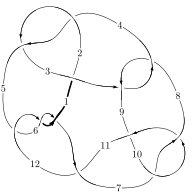
\includegraphics[width=112pt]{../../../GIT/diagram.site/Diagrams/png/967_12a_0166.png}\\
\ \ \ A knot diagram\footnotemark}&
\allowdisplaybreaks
\textbf{Linearized knot diagam} \\
\cline{2-2}
 &
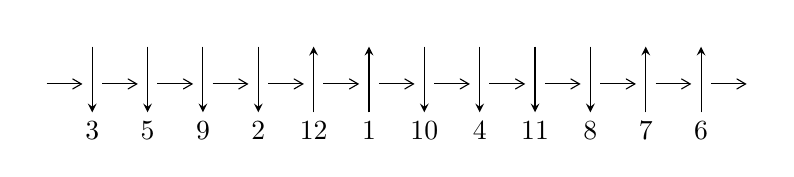
\begin{tikzpicture}[x=20pt, y=17pt]
	% nodes
	\node (C0) at (0, 0) {};
	\node (C1) at (1, 0) {};
	\node (C1U) at (1, +1) {};
	\node (C1D) at (1, -1) {3};

	\node (C2) at (2, 0) {};
	\node (C2U) at (2, +1) {};
	\node (C2D) at (2, -1) {5};

	\node (C3) at (3, 0) {};
	\node (C3U) at (3, +1) {};
	\node (C3D) at (3, -1) {9};

	\node (C4) at (4, 0) {};
	\node (C4U) at (4, +1) {};
	\node (C4D) at (4, -1) {2};

	\node (C5) at (5, 0) {};
	\node (C5U) at (5, +1) {};
	\node (C5D) at (5, -1) {12};

	\node (C6) at (6, 0) {};
	\node (C6U) at (6, +1) {};
	\node (C6D) at (6, -1) {1};

	\node (C7) at (7, 0) {};
	\node (C7U) at (7, +1) {};
	\node (C7D) at (7, -1) {10};

	\node (C8) at (8, 0) {};
	\node (C8U) at (8, +1) {};
	\node (C8D) at (8, -1) {4};

	\node (C9) at (9, 0) {};
	\node (C9U) at (9, +1) {};
	\node (C9D) at (9, -1) {11};

	\node (C10) at (10, 0) {};
	\node (C10U) at (10, +1) {};
	\node (C10D) at (10, -1) {8};

	\node (C11) at (11, 0) {};
	\node (C11U) at (11, +1) {};
	\node (C11D) at (11, -1) {7};

	\node (C12) at (12, 0) {};
	\node (C12U) at (12, +1) {};
	\node (C12D) at (12, -1) {6};
	\node (C13) at (13, 0) {};

	% arrows
	\draw[->,>={angle 60}]
	(C0) edge (C1) (C1) edge (C2) (C2) edge (C3) (C3) edge (C4) (C4) edge (C5) (C5) edge (C6) (C6) edge (C7) (C7) edge (C8) (C8) edge (C9) (C9) edge (C10) (C10) edge (C11) (C11) edge (C12) (C12) edge (C13) ;	\draw[->,>=stealth]
	(C1U) edge (C1D) (C2U) edge (C2D) (C3U) edge (C3D) (C4U) edge (C4D) (C5D) edge (C5U) (C6D) edge (C6U) (C7U) edge (C7D) (C8U) edge (C8D) (C9U) edge (C9D) (C10U) edge (C10D) (C11D) edge (C11U) (C12D) edge (C12U) ;
	\end{tikzpicture} \\
\hhline{~~} \\& 
\textbf{Solving Sequence} \\ \cline{2-2} 
 &
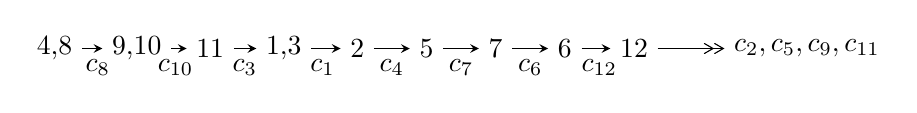
\begin{tikzpicture}[x=25pt, y=7pt]
	% node
	\node (A0) at (-1/8, 0) {4,8};
	\node (A1) at (17/16, 0) {9,10};
	\node (A2) at (17/8, 0) {11};
	\node (A3) at (51/16, 0) {1,3};
	\node (A4) at (17/4, 0) {2};
	\node (A5) at (21/4, 0) {5};
	\node (A6) at (25/4, 0) {7};
	\node (A7) at (29/4, 0) {6};
	\node (A8) at (33/4, 0) {12};
	\node (C1) at (1/2, -1) {$c_{8}$};
	\node (C2) at (13/8, -1) {$c_{10}$};
	\node (C3) at (21/8, -1) {$c_{3}$};
	\node (C4) at (15/4, -1) {$c_{1}$};
	\node (C5) at (19/4, -1) {$c_{4}$};
	\node (C6) at (23/4, -1) {$c_{7}$};
	\node (C7) at (27/4, -1) {$c_{6}$};
	\node (C8) at (31/4, -1) {$c_{12}$};
	\node (A9) at (43/4, 0) {$c_{2},c_{5},c_{9},c_{11}$};

	% edge
	\draw[->,>=stealth]	
	(A0) edge (A1) (A1) edge (A2) (A2) edge (A3) (A3) edge (A4) (A4) edge (A5) (A5) edge (A6) (A6) edge (A7) (A7) edge (A8) ;
	\draw[->>,>={angle 60}]	
	(A8) edge (A9);
\end{tikzpicture} \\ 

\end{tabular} \\

\footnotetext{
The image of knot diagram is generated by the software ``\textbf{Draw programme}" developed by Andrew Bartholomew(\url{http://www.layer8.co.uk/maths/draw/index.htm\#Running-draw}), where we modified some parts for our purpose(\url{https://github.com/CATsTAILs/LinksPainter}).
}\phantom \\ \newline 
\centering \textbf{Ideals for irreducible components\footnotemark of $X_{\text{par}}$} 
 
\begin{align*}
I^u_{1}&=\langle 
458802669672 u^{24}+367351897733 u^{23}+\cdots+7058049605558 d-1244576019090,\\
\phantom{I^u_{1}}&\phantom{= \langle  }147880761515 u^{24}-335144114156 u^{23}+\cdots+28232198422232 c-35621876846456,\\
\phantom{I^u_{1}}&\phantom{= \langle  }1278289196883 u^{24}+1997820239306 u^{23}+\cdots+14116099211116 b-10424467040404,\\
\phantom{I^u_{1}}&\phantom{= \langle  }377943683179 u^{24}+896277965838 u^{23}+\cdots+28232198422232 a-14859817453240,\\
\phantom{I^u_{1}}&\phantom{= \langle  }u^{25}+2 u^{24}+\cdots-16 u-8\rangle \\
I^u_{2}&=\langle 
2 u^{10} a- u^{10}+\cdots-6 a-7,\;10 u^{10} a+5 u^{10}+\cdots-18 a-34,\;2 u^9 a+3 u^{10}+\cdots+b+2 a,\\
\phantom{I^u_{2}}&\phantom{= \langle  }3 u^{10} a+8 u^{10}+\cdots+2 a^2-6,\;u^{11}-3 u^{10}+6 u^9-7 u^8+7 u^7-3 u^6-2 u^5+8 u^4-7 u^3+5 u^2-2 u+2\rangle \\
I^u_{3}&=\langle 
- u^7- u^5-2 u^3+d- u,\;- u^7-2 u^5-2 u^3+c-2 u,\;u^8 a+25 u^8+\cdots-28 a+13,\\
\phantom{I^u_{3}}&\phantom{= \langle  }- u^8-2 u^7-3 u^6-3 u^5-3 u^4+u^2 a-2 u^3+a^2+2 a u-3 u^2+a,\\
\phantom{I^u_{3}}&\phantom{= \langle  }u^9+u^8+2 u^7+u^6+3 u^5+u^4+2 u^3+u-1\rangle \\
I^u_{4}&=\langle 
u^8 c+5 u^8+\cdots-27 c+10,\;2 u^8 c-2 u^8+\cdots+2 c-4,\;- u^2+b,\;- u^2+a-1,\\
\phantom{I^u_{4}}&\phantom{= \langle  }u^9+u^8+2 u^7+u^6+3 u^5+u^4+2 u^3+u-1\rangle \\
I^u_{5}&=\langle 
- u^7- u^5-2 u^3+d- u,\;- u^7-2 u^5-2 u^3+c-2 u,\;- u^2+b,\;- u^2+a-1,\\
\phantom{I^u_{5}}&\phantom{= \langle  }u^9+u^8+2 u^7+u^6+3 u^5+u^4+2 u^3+u-1\rangle \\
\\
I^v_{1}&=\langle 
a,\;d-1,\;c- a-1,\;b-1,\;v+1\rangle \\
I^v_{2}&=\langle 
a,\;d,\;c-1,\;b+1,\;v-1\rangle \\
I^v_{3}&=\langle 
c,\;d-1,\;b,\;a-1,\;v-1\rangle \\
I^v_{4}&=\langle 
c,\;d-1,\;a v+c- v-1,\;b v+1\rangle \\
\end{align*}
\raggedright * 8 irreducible components of $\dim_{\mathbb{C}}=0$, with total 95 representations.\\
\raggedright * 1 irreducible components of $\dim_{\mathbb{C}}=1$ \\
\footnotetext{All coefficients of polynomials are rational numbers. But the coefficients are sometimes approximated in decimal forms when there is not enough margin.}
\newpage
\renewcommand{\arraystretch}{1}
\centering \section*{I. $I^u_{1}= \langle 4.59\times10^{11} u^{24}+3.67\times10^{11} u^{23}+\cdots+7.06\times10^{12} d-1.24\times10^{12},\;1.48\times10^{11} u^{24}-3.35\times10^{11} u^{23}+\cdots+2.82\times10^{13} c-3.56\times10^{13},\;1.28\times10^{12} u^{24}+2.00\times10^{12} u^{23}+\cdots+1.41\times10^{13} b-1.04\times10^{13},\;3.78\times10^{11} u^{24}+8.96\times10^{11} u^{23}+\cdots+2.82\times10^{13} a-1.49\times10^{13},\;u^{25}+2 u^{24}+\cdots-16 u-8 \rangle$}
\flushleft \textbf{(i) Arc colorings}\\
\begin{tabular}{m{7pt} m{180pt} m{7pt} m{180pt} }
\flushright $a_{4}=$&$\begin{pmatrix}0\\u\end{pmatrix}$ \\
\flushright $a_{8}=$&$\begin{pmatrix}1\\0\end{pmatrix}$ \\
\flushright $a_{9}=$&$\begin{pmatrix}1\\u^2\end{pmatrix}$ \\
\flushright $a_{10}=$&$\begin{pmatrix}-0.00523802 u^{24}+0.0118710 u^{23}+\cdots+0.471795 u+1.26175\\-0.0650042 u^{24}-0.0520472 u^{23}+\cdots+0.578878 u+0.176334\end{pmatrix}$ \\
\flushright $a_{11}=$&$\begin{pmatrix}0.0597662 u^{24}+0.0639182 u^{23}+\cdots-0.107083 u+1.08541\\-0.0650042 u^{24}-0.0520472 u^{23}+\cdots+0.578878 u+0.176334\end{pmatrix}$ \\
\flushright $a_{1}=$&$\begin{pmatrix}-0.0133870 u^{24}-0.0317467 u^{23}+\cdots+1.11820 u+0.526343\\-0.0905554 u^{24}-0.141528 u^{23}+\cdots+1.83403 u+0.738481\end{pmatrix}$ \\
\flushright $a_{3}=$&$\begin{pmatrix}u\\u^3+u\end{pmatrix}$ \\
\flushright $a_{2}=$&$\begin{pmatrix}0.0220418 u^{24}-0.0209206 u^{23}+\cdots+1.13918 u+0.226210\\0.0223470 u^{24}-0.0180859 u^{23}+\cdots+1.17794 u-0.0419041\end{pmatrix}$ \\
\flushright $a_{5}=$&$\begin{pmatrix}-0.0776559 u^{24}-0.117795 u^{23}+\cdots+0.902489 u+0.251920\\-0.0910429 u^{24}-0.149542 u^{23}+\cdots+2.02069 u+0.778262\end{pmatrix}$ \\
\flushright $a_{7}=$&$\begin{pmatrix}0.0972828 u^{24}+0.103523 u^{23}+\cdots-1.09766 u+0.464165\\0.0375166 u^{24}+0.0396045 u^{23}+\cdots-0.990575 u-0.621247\end{pmatrix}$ \\
\flushright $a_{6}=$&$\begin{pmatrix}0.151545 u^{24}+0.183512 u^{23}+\cdots-2.01089 u-0.346355\\0.119577 u^{24}+0.131747 u^{23}+\cdots-2.07836 u-1.21236\end{pmatrix}$ \\
\flushright $a_{12}=$&$\begin{pmatrix}0.0923101 u^{24}+0.0940648 u^{23}+\cdots-0.785506 u+0.357069\\-0.00497271 u^{24}-0.00945799 u^{23}+\cdots+0.312151 u-0.107096\end{pmatrix}$\\&\end{tabular}
\flushleft \textbf{(ii) Obstruction class $= -1$}\\~\\
\flushleft \textbf{(iii) Cusp Shapes $= \frac{8058725701665}{7058049605558} u^{24}+\frac{10736954342885}{7058049605558} u^{23}+\cdots-\frac{38478403451674}{3529024802779} u-\frac{29622418287164}{3529024802779}$}\\~\\
\newpage\renewcommand{\arraystretch}{1}
\flushleft \textbf{(iv) u-Polynomials at the component}\newline \\
\begin{tabular}{m{50pt}|m{274pt}}
Crossings & \hspace{64pt}u-Polynomials at each crossing \\
\hline $$\begin{aligned}c_{1},c_{9}\end{aligned}$$&$\begin{aligned}
&u^{25}+12 u^{24}+\cdots+3 u+1
\end{aligned}$\\
\hline $$\begin{aligned}c_{2},c_{4},c_{7}\\c_{10}\end{aligned}$$&$\begin{aligned}
&u^{25}-2 u^{24}+\cdots- u+1
\end{aligned}$\\
\hline $$\begin{aligned}c_{3},c_{8}\end{aligned}$$&$\begin{aligned}
&u^{25}-2 u^{24}+\cdots-16 u+8
\end{aligned}$\\
\hline $$\begin{aligned}c_{5},c_{6},c_{12}\end{aligned}$$&$\begin{aligned}
&u^{25}+2 u^{24}+\cdots+8 u+4
\end{aligned}$\\
\hline $$\begin{aligned}c_{11}\end{aligned}$$&$\begin{aligned}
&u^{25}-6 u^{24}+\cdots+64 u+64
\end{aligned}$\\
\hline
\end{tabular}\\~\\
\newpage\renewcommand{\arraystretch}{1}
\flushleft \textbf{(v) Riley Polynomials at the component}\newline \\
\begin{tabular}{m{50pt}|m{274pt}}
Crossings & \hspace{64pt}Riley Polynomials at each crossing \\
\hline $$\begin{aligned}c_{1},c_{9}\end{aligned}$$&$\begin{aligned}
&y^{25}+8 y^{24}+\cdots-13 y-1
\end{aligned}$\\
\hline $$\begin{aligned}c_{2},c_{4},c_{7}\\c_{10}\end{aligned}$$&$\begin{aligned}
&y^{25}-12 y^{24}+\cdots+3 y-1
\end{aligned}$\\
\hline $$\begin{aligned}c_{3},c_{8}\end{aligned}$$&$\begin{aligned}
&y^{25}+6 y^{24}+\cdots+64 y-64
\end{aligned}$\\
\hline $$\begin{aligned}c_{5},c_{6},c_{12}\end{aligned}$$&$\begin{aligned}
&y^{25}-22 y^{24}+\cdots+88 y-16
\end{aligned}$\\
\hline $$\begin{aligned}c_{11}\end{aligned}$$&$\begin{aligned}
&y^{25}+14 y^{24}+\cdots+43008 y-4096
\end{aligned}$\\
\hline
\end{tabular}\\~\\
\newpage\flushleft \textbf{(vi) Complex Volumes and Cusp Shapes}
$$\begin{array}{c|c|c}  
\text{Solutions to }I^u_{1}& \I (\text{vol} + \sqrt{-1}CS) & \text{Cusp shape}\\
 \hline 
\begin{aligned}
u &= \phantom{-}1.041130 + 0.234144 I \\
a &= \phantom{-}0.008394 + 0.208390 I \\
b &= -0.269928 + 1.383510 I \\
c &= \phantom{-}1.348140 - 0.409095 I \\
d &= \phantom{-}0.853442 - 0.558038 I\end{aligned}
 & \phantom{-}3.14377 + 4.46824 I & -1.00511 - 6.27335 I \\ \hline\begin{aligned}
u &= \phantom{-}1.041130 - 0.234144 I \\
a &= \phantom{-}0.008394 - 0.208390 I \\
b &= -0.269928 - 1.383510 I \\
c &= \phantom{-}1.348140 + 0.409095 I \\
d &= \phantom{-}0.853442 + 0.558038 I\end{aligned}
 & \phantom{-}3.14377 - 4.46824 I & -1.00511 + 6.27335 I \\ \hline\begin{aligned}
u &= -0.804646 + 0.457350 I \\
a &= -0.895367 + 0.386742 I \\
b &= -1.161700 + 0.803797 I \\
c &= \phantom{-}0.875912 - 0.274270 I \\
d &= \phantom{-}0.214886 - 0.601608 I\end{aligned}
 & \phantom{-}2.41327 - 0.90505 I & \phantom{-}1.24488 - 0.76686 I \\ \hline\begin{aligned}
u &= -0.804646 - 0.457350 I \\
a &= -0.895367 - 0.386742 I \\
b &= -1.161700 - 0.803797 I \\
c &= \phantom{-}0.875912 + 0.274270 I \\
d &= \phantom{-}0.214886 + 0.601608 I\end{aligned}
 & \phantom{-}2.41327 + 0.90505 I & \phantom{-}1.24488 + 0.76686 I \\ \hline\begin{aligned}
u &= -0.336133 + 1.048560 I \\
a &= -0.156441 - 0.276251 I \\
b &= \phantom{-}0.845749 + 0.298371 I \\
c &= -0.694150 - 1.216860 I \\
d &= -0.927060 + 0.554841 I\end{aligned}
 & \phantom{-}0.70247 + 6.59785 I & -2.96140 - 9.56947 I \\ \hline\begin{aligned}
u &= -0.336133 - 1.048560 I \\
a &= -0.156441 + 0.276251 I \\
b &= \phantom{-}0.845749 - 0.298371 I \\
c &= -0.694150 + 1.216860 I \\
d &= -0.927060 - 0.554841 I\end{aligned}
 & \phantom{-}0.70247 - 6.59785 I & -2.96140 + 9.56947 I\\
 \hline 
 \end{array}$$\newpage$$\begin{array}{c|c|c}  
\text{Solutions to }I^u_{1}& \I (\text{vol} + \sqrt{-1}CS) & \text{Cusp shape}\\
 \hline 
\begin{aligned}
u &= \phantom{-}0.926049 + 0.758012 I \\
a &= -1.42251 - 0.81155 I \\
b &= -0.87316 - 1.69108 I \\
c &= \phantom{-}1.62524 - 0.37230 I \\
d &= \phantom{-}1.187970 - 0.465287 I\end{aligned}
 & -7.68831 + 5.75962 I & -10.13195 - 4.49272 I \\ \hline\begin{aligned}
u &= \phantom{-}0.926049 - 0.758012 I \\
a &= -1.42251 + 0.81155 I \\
b &= -0.87316 + 1.69108 I \\
c &= \phantom{-}1.62524 + 0.37230 I \\
d &= \phantom{-}1.187970 + 0.465287 I\end{aligned}
 & -7.68831 - 5.75962 I & -10.13195 + 4.49272 I \\ \hline\begin{aligned}
u &= -0.759240 + 0.251838 I \\
a &= -0.264762 - 0.457484 I \\
b &= -0.051945 + 0.352201 I \\
c &= \phantom{-}1.384510 + 0.243604 I \\
d &= \phantom{-}0.865432 + 0.337523 I\end{aligned}
 & -2.09943 - 2.64913 I & -8.26724 + 7.08829 I \\ \hline\begin{aligned}
u &= -0.759240 - 0.251838 I \\
a &= -0.264762 + 0.457484 I \\
b &= -0.051945 - 0.352201 I \\
c &= \phantom{-}1.384510 - 0.243604 I \\
d &= \phantom{-}0.865432 - 0.337523 I\end{aligned}
 & -2.09943 + 2.64913 I & -8.26724 - 7.08829 I \\ \hline\begin{aligned}
u &= -0.169266 + 0.764490 I \\
a &= -0.128013 + 0.686745 I \\
b &= -0.303623 + 0.446468 I \\
c &= \phantom{-}0.734127 + 0.404802 I \\
d &= -0.420684 - 0.407489 I\end{aligned}
 & \phantom{-}1.62680 - 1.08260 I & \phantom{-}3.35440 + 3.89731 I \\ \hline\begin{aligned}
u &= -0.169266 - 0.764490 I \\
a &= -0.128013 - 0.686745 I \\
b &= -0.303623 - 0.446468 I \\
c &= \phantom{-}0.734127 - 0.404802 I \\
d &= -0.420684 + 0.407489 I\end{aligned}
 & \phantom{-}1.62680 + 1.08260 I & \phantom{-}3.35440 - 3.89731 I\\
 \hline 
 \end{array}$$\newpage$$\begin{array}{c|c|c}  
\text{Solutions to }I^u_{1}& \I (\text{vol} + \sqrt{-1}CS) & \text{Cusp shape}\\
 \hline 
\begin{aligned}
u &= \phantom{-}0.096683 + 1.217070 I \\
a &= -0.596071 + 0.850107 I \\
b &= \phantom{-}0.883990 - 0.599145 I \\
c &= -0.133481 - 0.336989 I \\
d &= -0.646064 + 0.751814 I\end{aligned}
 & \phantom{-}8.85704 + 0.98974 I & \phantom{-}4.51267 - 2.53049 I \\ \hline\begin{aligned}
u &= \phantom{-}0.096683 - 1.217070 I \\
a &= -0.596071 - 0.850107 I \\
b &= \phantom{-}0.883990 + 0.599145 I \\
c &= -0.133481 + 0.336989 I \\
d &= -0.646064 - 0.751814 I\end{aligned}
 & \phantom{-}8.85704 - 0.98974 I & \phantom{-}4.51267 + 2.53049 I \\ \hline\begin{aligned}
u &= -0.661369 + 1.057320 I \\
a &= -0.57589 + 1.50124 I \\
b &= \phantom{-}1.36579 + 0.96216 I \\
c &= \phantom{-}0.362414 - 0.234138 I \\
d &= -0.212320 - 0.866068 I\end{aligned}
 & \phantom{-}4.06909 + 6.32284 I & \phantom{-}1.86961 - 4.09954 I \\ \hline\begin{aligned}
u &= -0.661369 - 1.057320 I \\
a &= -0.57589 - 1.50124 I \\
b &= \phantom{-}1.36579 - 0.96216 I \\
c &= \phantom{-}0.362414 + 0.234138 I \\
d &= -0.212320 + 0.866068 I\end{aligned}
 & \phantom{-}4.06909 - 6.32284 I & \phantom{-}1.86961 + 4.09954 I \\ \hline\begin{aligned}
u &= -1.024310 + 0.754591 I \\
a &= \phantom{-}1.59421 - 0.47481 I \\
b &= \phantom{-}1.76886 - 1.85122 I \\
c &= \phantom{-}1.62073 + 0.41845 I \\
d &= \phantom{-}1.188320 + 0.521494 I\end{aligned}
 & -3.22783 - 10.10170 I & -5.60475 + 6.88322 I \\ \hline\begin{aligned}
u &= -1.024310 - 0.754591 I \\
a &= \phantom{-}1.59421 + 0.47481 I \\
b &= \phantom{-}1.76886 + 1.85122 I \\
c &= \phantom{-}1.62073 - 0.41845 I \\
d &= \phantom{-}1.188320 - 0.521494 I\end{aligned}
 & -3.22783 + 10.10170 I & -5.60475 - 6.88322 I\\
 \hline 
 \end{array}$$\newpage$$\begin{array}{c|c|c}  
\text{Solutions to }I^u_{1}& \I (\text{vol} + \sqrt{-1}CS) & \text{Cusp shape}\\
 \hline 
\begin{aligned}
u &= \phantom{-}0.425565 + 1.220260 I \\
a &= \phantom{-}0.635489 - 0.691012 I \\
b &= -0.588986 + 0.949659 I \\
c &= -1.004750 + 0.853367 I \\
d &= -1.001440 - 0.660540 I\end{aligned}
 & \phantom{-}6.70868 - 9.75196 I & \phantom{-}0.64851 + 8.69449 I \\ \hline\begin{aligned}
u &= \phantom{-}0.425565 - 1.220260 I \\
a &= \phantom{-}0.635489 + 0.691012 I \\
b &= -0.588986 - 0.949659 I \\
c &= -1.004750 - 0.853367 I \\
d &= -1.001440 + 0.660540 I\end{aligned}
 & \phantom{-}6.70868 + 9.75196 I & \phantom{-}0.64851 - 8.69449 I \\ \hline\begin{aligned}
u &= \phantom{-}0.797713 + 1.033120 I \\
a &= -0.52447 - 1.76199 I \\
b &= \phantom{-}1.27330 - 1.73823 I \\
c &= -1.87693 + 1.11019 I \\
d &= -1.213130 - 0.525024 I\end{aligned}
 & -6.80818 - 12.11480 I & -8.50713 + 8.67244 I \\ \hline\begin{aligned}
u &= \phantom{-}0.797713 - 1.033120 I \\
a &= -0.52447 + 1.76199 I \\
b &= \phantom{-}1.27330 + 1.73823 I \\
c &= -1.87693 - 1.11019 I \\
d &= -1.213130 + 0.525024 I\end{aligned}
 & -6.80818 + 12.11480 I & -8.50713 - 8.67244 I \\ \hline\begin{aligned}
u &= -0.832592 + 1.087810 I \\
a &= \phantom{-}0.39378 - 1.99462 I \\
b &= -2.07832 - 1.63190 I \\
c &= -1.88297 - 0.97500 I \\
d &= -1.234910 + 0.554337 I\end{aligned}
 & -2.1296 + 16.8657 I & -4.74649 - 10.33694 I \\ \hline\begin{aligned}
u &= -0.832592 - 1.087810 I \\
a &= \phantom{-}0.39378 + 1.99462 I \\
b &= -2.07832 + 1.63190 I \\
c &= -1.88297 + 0.97500 I \\
d &= -1.234910 - 0.554337 I\end{aligned}
 & -2.1296 - 16.8657 I & -4.74649 + 10.33694 I\\
 \hline 
 \end{array}$$\newpage$$\begin{array}{c|c|c}  
\text{Solutions to }I^u_{1}& \I (\text{vol} + \sqrt{-1}CS) & \text{Cusp shape}\\
 \hline 
\begin{aligned}
u &= \phantom{-}0.600838\phantom{ +0.000000I} \\
a &= \phantom{-}0.863277\phantom{ +0.000000I} \\
b &= \phantom{-}0.379944\phantom{ +0.000000I} \\
c &= \phantom{-}1.28245\phantom{ +0.000000I} \\
d &= \phantom{-}0.691126\phantom{ +0.000000I}\end{aligned}
 & -1.26593\phantom{ +0.000000I} & -6.81200\phantom{ +0.000000I}\\
 \hline 
 \end{array}$$\newpage\newpage\renewcommand{\arraystretch}{1}
\centering \section*{II. $I^u_{2}= \langle 2 u^{10} a- u^{10}+\cdots-6 a-7,\;10 u^{10} a+5 u^{10}+\cdots-18 a-34,\;2 u^9 a+3 u^{10}+\cdots+b+2 a,\;3 u^{10} a+8 u^{10}+\cdots+2 a^2-6,\;u^{11}-3 u^{10}+\cdots-2 u+2 \rangle$}
\flushleft \textbf{(i) Arc colorings}\\
\begin{tabular}{m{7pt} m{180pt} m{7pt} m{180pt} }
\flushright $a_{4}=$&$\begin{pmatrix}0\\u\end{pmatrix}$ \\
\flushright $a_{8}=$&$\begin{pmatrix}1\\0\end{pmatrix}$ \\
\flushright $a_{9}=$&$\begin{pmatrix}1\\u^2\end{pmatrix}$ \\
\flushright $a_{10}=$&$\begin{pmatrix}-5 u^{10} a-\frac{5}{2} u^{10}+\cdots+9 a+17\\-2 u^{10} a+u^{10}+\cdots+6 a+7\end{pmatrix}$ \\
\flushright $a_{11}=$&$\begin{pmatrix}-3 u^{10} a-\frac{7}{2} u^{10}+\cdots+3 a+10\\-2 u^{10} a+u^{10}+\cdots+6 a+7\end{pmatrix}$ \\
\flushright $a_{1}=$&$\begin{pmatrix}a\\-2 u^9 a-3 u^{10}+\cdots-2 a-3 u\end{pmatrix}$ \\
\flushright $a_{3}=$&$\begin{pmatrix}u\\u^3+u\end{pmatrix}$ \\
\flushright $a_{2}=$&$\begin{pmatrix}3 u^{10} a+3 u^{10}+\cdots-3 a-10\\2 u^{10} a-7 u^{10}+\cdots-10 a-6\end{pmatrix}$ \\
\flushright $a_{5}=$&$\begin{pmatrix}-2 u^9 a-3 u^{10}+\cdots-3 a-3 u\\-2 u^9 a-3 u^{10}+\cdots-2 a-3 u\end{pmatrix}$ \\
\flushright $a_{7}=$&$\begin{pmatrix}- u^{10} a+\frac{3}{2} u^{10}+\cdots+3 a+1\\2 u^{10} a+5 u^{10}+\cdots+6 u-9\end{pmatrix}$ \\
\flushright $a_{6}=$&$\begin{pmatrix}u^9 a+\frac{3}{2} u^{10}+\cdots+2 a+1\\u^{10} a+3 u^{10}+\cdots+3 u-3\end{pmatrix}$ \\
\flushright $a_{12}=$&$\begin{pmatrix}- u^{10} a-\frac{3}{2} u^{10}+\cdots+3 a+4\\-3 u^{10}+6 u^9+\cdots-3 u+3\end{pmatrix}$\\&\end{tabular}
\flushleft \textbf{(ii) Obstruction class $= -1$}\\~\\
\flushleft \textbf{(iii) Cusp Shapes $= 2 u^{10}-8 u^9+10 u^8-10 u^7+4 u^6-4 u^5-14 u^4+12 u^3-6 u^2-8 u-12$}\\~\\
\newpage\renewcommand{\arraystretch}{1}
\flushleft \textbf{(iv) u-Polynomials at the component}\newline \\
\begin{tabular}{m{50pt}|m{274pt}}
Crossings & \hspace{64pt}u-Polynomials at each crossing \\
\hline $$\begin{aligned}c_{1},c_{9}\end{aligned}$$&$\begin{aligned}
&u^{22}+11 u^{21}+\cdots+40 u+16
\end{aligned}$\\
\hline $$\begin{aligned}c_{2},c_{4},c_{7}\\c_{10}\end{aligned}$$&$\begin{aligned}
&u^{22}- u^{21}+\cdots-4 u+4
\end{aligned}$\\
\hline $$\begin{aligned}c_{3},c_{8}\end{aligned}$$&$\begin{aligned}
&(u^{11}+3 u^{10}+6 u^9+7 u^8+7 u^7+3 u^6-2 u^5-8 u^4-7 u^3-5 u^2-2 u-2)^{2}
\end{aligned}$\\
\hline $$\begin{aligned}c_{5},c_{6},c_{12}\end{aligned}$$&$\begin{aligned}
&(u^{11}+u^{10}-5 u^9-4 u^8+9 u^7+4 u^6-5 u^5+3 u^4-3 u^3-5 u^2+3 u-1)^2
\end{aligned}$\\
\hline $$\begin{aligned}c_{11}\end{aligned}$$&$\begin{aligned}
&(u^{11}-3 u^{10}+\cdots-16 u+4)^{2}
\end{aligned}$\\
\hline
\end{tabular}\\~\\
\newpage\renewcommand{\arraystretch}{1}
\flushleft \textbf{(v) Riley Polynomials at the component}\newline \\
\begin{tabular}{m{50pt}|m{274pt}}
Crossings & \hspace{64pt}Riley Polynomials at each crossing \\
\hline $$\begin{aligned}c_{1},c_{9}\end{aligned}$$&$\begin{aligned}
&y^{22}-3 y^{21}+\cdots-544 y+256
\end{aligned}$\\
\hline $$\begin{aligned}c_{2},c_{4},c_{7}\\c_{10}\end{aligned}$$&$\begin{aligned}
&y^{22}-11 y^{21}+\cdots-40 y+16
\end{aligned}$\\
\hline $$\begin{aligned}c_{3},c_{8}\end{aligned}$$&$\begin{aligned}
&(y^{11}+3 y^{10}+\cdots-16 y-4)^{2}
\end{aligned}$\\
\hline $$\begin{aligned}c_{5},c_{6},c_{12}\end{aligned}$$&$\begin{aligned}
&(y^{11}-11 y^{10}+\cdots- y-1)^{2}
\end{aligned}$\\
\hline $$\begin{aligned}c_{11}\end{aligned}$$&$\begin{aligned}
&(y^{11}+7 y^{10}+\cdots+24 y-16)^{2}
\end{aligned}$\\
\hline
\end{tabular}\\~\\
\newpage\flushleft \textbf{(vi) Complex Volumes and Cusp Shapes}
$$\begin{array}{c|c|c}  
\text{Solutions to }I^u_{2}& \I (\text{vol} + \sqrt{-1}CS) & \text{Cusp shape}\\
 \hline 
\begin{aligned}
u &= -0.992754\phantom{ +0.000000I} \\
a &= -0.539348 + 0.169351 I \\
b &= -0.94293 + 1.07661 I \\
c &= \phantom{-}1.202080 - 0.374899 I \\
d &= \phantom{-}0.660661 - 0.556253 I\end{aligned}
 & \phantom{-}3.69004\phantom{ +0.000000I} & \phantom{-}0.666830\phantom{ +0.000000I} \\ \hline\begin{aligned}
u &= -0.992754\phantom{ +0.000000I} \\
a &= -0.539348 - 0.169351 I \\
b &= -0.94293 - 1.07661 I \\
c &= \phantom{-}1.202080 + 0.374899 I \\
d &= \phantom{-}0.660661 + 0.556253 I\end{aligned}
 & \phantom{-}3.69004\phantom{ +0.000000I} & \phantom{-}0.666830\phantom{ +0.000000I} \\ \hline\begin{aligned}
u &= \phantom{-}0.762686 + 0.875309 I \\
a &= -0.98257 - 1.33960 I \\
b &= -0.38116 - 2.19608 I \\
c &= \phantom{-}1.68434 - 0.30273 I \\
d &= \phantom{-}1.252300 - 0.374583 I\end{aligned}
 & -7.89368 - 2.87937 I & -10.41286 + 3.23335 I \\ \hline\begin{aligned}
u &= \phantom{-}0.762686 + 0.875309 I \\
a &= -1.44491 - 1.55956 I \\
b &= \phantom{-}0.70519 - 1.74288 I \\
c &= -2.02916 + 1.48909 I \\
d &= -1.190170 - 0.436468 I\end{aligned}
 & -7.89368 - 2.87937 I & -10.41286 + 3.23335 I \\ \hline\begin{aligned}
u &= \phantom{-}0.762686 - 0.875309 I \\
a &= -0.98257 + 1.33960 I \\
b &= -0.38116 + 2.19608 I \\
c &= \phantom{-}1.68434 + 0.30273 I \\
d &= \phantom{-}1.252300 + 0.374583 I\end{aligned}
 & -7.89368 + 2.87937 I & -10.41286 - 3.23335 I \\ \hline\begin{aligned}
u &= \phantom{-}0.762686 - 0.875309 I \\
a &= -1.44491 + 1.55956 I \\
b &= \phantom{-}0.70519 + 1.74288 I \\
c &= -2.02916 - 1.48909 I \\
d &= -1.190170 + 0.436468 I\end{aligned}
 & -7.89368 + 2.87937 I & -10.41286 - 3.23335 I\\
 \hline 
 \end{array}$$\newpage$$\begin{array}{c|c|c}  
\text{Solutions to }I^u_{2}& \I (\text{vol} + \sqrt{-1}CS) & \text{Cusp shape}\\
 \hline 
\begin{aligned}
u &= \phantom{-}0.958422 + 0.661375 I \\
a &= -1.166710 - 0.533776 I \\
b &= -1.25478 - 0.98207 I \\
c &= \phantom{-}0.744407 + 0.405064 I \\
d &= \phantom{-}0.164345 + 0.807203 I\end{aligned}
 & -0.20533 + 5.20915 I & -2.55774 - 3.72118 I \\ \hline\begin{aligned}
u &= \phantom{-}0.958422 + 0.661375 I \\
a &= \phantom{-}1.28394 + 0.64916 I \\
b &= \phantom{-}1.39078 + 2.09707 I \\
c &= \phantom{-}1.57823 - 0.38401 I \\
d &= \phantom{-}1.132380 - 0.485520 I\end{aligned}
 & -0.20533 + 5.20915 I & -2.55774 - 3.72118 I \\ \hline\begin{aligned}
u &= \phantom{-}0.958422 - 0.661375 I \\
a &= -1.166710 + 0.533776 I \\
b &= -1.25478 + 0.98207 I \\
c &= \phantom{-}0.744407 - 0.405064 I \\
d &= \phantom{-}0.164345 - 0.807203 I\end{aligned}
 & -0.20533 - 5.20915 I & -2.55774 + 3.72118 I \\ \hline\begin{aligned}
u &= \phantom{-}0.958422 - 0.661375 I \\
a &= \phantom{-}1.28394 - 0.64916 I \\
b &= \phantom{-}1.39078 - 2.09707 I \\
c &= \phantom{-}1.57823 + 0.38401 I \\
d &= \phantom{-}1.132380 + 0.485520 I\end{aligned}
 & -0.20533 - 5.20915 I & -2.55774 + 3.72118 I \\ \hline\begin{aligned}
u &= -0.273627 + 1.210650 I \\
a &= \phantom{-}0.376337 + 1.232810 I \\
b &= -0.055892 - 0.873986 I \\
c &= -0.687715 - 0.784193 I \\
d &= -0.901383 + 0.672173 I\end{aligned}
 & \phantom{-}8.10965 + 4.33574 I & \phantom{-}3.31243 - 3.68401 I \\ \hline\begin{aligned}
u &= -0.273627 + 1.210650 I \\
a &= -0.680000 - 0.179254 I \\
b &= \phantom{-}1.163320 + 0.588782 I \\
c &= \phantom{-}0.0243773 + 0.1172880 I \\
d &= -0.522674 - 0.802934 I\end{aligned}
 & \phantom{-}8.10965 + 4.33574 I & \phantom{-}3.31243 - 3.68401 I\\
 \hline 
 \end{array}$$\newpage$$\begin{array}{c|c|c}  
\text{Solutions to }I^u_{2}& \I (\text{vol} + \sqrt{-1}CS) & \text{Cusp shape}\\
 \hline 
\begin{aligned}
u &= -0.273627 - 1.210650 I \\
a &= \phantom{-}0.376337 - 1.232810 I \\
b &= -0.055892 + 0.873986 I \\
c &= -0.687715 + 0.784193 I \\
d &= -0.901383 - 0.672173 I\end{aligned}
 & \phantom{-}8.10965 - 4.33574 I & \phantom{-}3.31243 + 3.68401 I \\ \hline\begin{aligned}
u &= -0.273627 - 1.210650 I \\
a &= -0.680000 + 0.179254 I \\
b &= \phantom{-}1.163320 - 0.588782 I \\
c &= \phantom{-}0.0243773 - 0.1172880 I \\
d &= -0.522674 + 0.802934 I\end{aligned}
 & \phantom{-}8.10965 - 4.33574 I & \phantom{-}3.31243 + 3.68401 I \\ \hline\begin{aligned}
u &= \phantom{-}0.764438 + 1.080520 I \\
a &= -0.29279 - 1.73056 I \\
b &= \phantom{-}1.42979 - 1.08893 I \\
c &= \phantom{-}0.371944 + 0.333066 I \\
d &= -0.163987 + 0.927905 I\end{aligned}
 & \phantom{-}1.11929 - 11.51290 I & -1.55919 + 7.44023 I \\ \hline\begin{aligned}
u &= \phantom{-}0.764438 + 1.080520 I \\
a &= \phantom{-}0.80955 + 1.63996 I \\
b &= -1.82005 + 1.63929 I \\
c &= -1.76532 + 1.05251 I \\
d &= -1.196120 - 0.553243 I\end{aligned}
 & \phantom{-}1.11929 - 11.51290 I & -1.55919 + 7.44023 I \\ \hline\begin{aligned}
u &= \phantom{-}0.764438 - 1.080520 I \\
a &= -0.29279 + 1.73056 I \\
b &= \phantom{-}1.42979 + 1.08893 I \\
c &= \phantom{-}0.371944 - 0.333066 I \\
d &= -0.163987 - 0.927905 I\end{aligned}
 & \phantom{-}1.11929 + 11.51290 I & -1.55919 - 7.44023 I \\ \hline\begin{aligned}
u &= \phantom{-}0.764438 - 1.080520 I \\
a &= \phantom{-}0.80955 - 1.63996 I \\
b &= -1.82005 - 1.63929 I \\
c &= -1.76532 - 1.05251 I \\
d &= -1.196120 + 0.553243 I\end{aligned}
 & \phantom{-}1.11929 + 11.51290 I & -1.55919 - 7.44023 I\\
 \hline 
 \end{array}$$\newpage$$\begin{array}{c|c|c}  
\text{Solutions to }I^u_{2}& \I (\text{vol} + \sqrt{-1}CS) & \text{Cusp shape}\\
 \hline 
\begin{aligned}
u &= -0.215541 + 0.601634 I \\
a &= \phantom{-}0.704776 + 0.667690 I \\
b &= \phantom{-}1.56963 + 1.15126 I \\
c &= \phantom{-}1.60686 + 0.07009 I \\
d &= \phantom{-}1.140500 + 0.089613 I\end{aligned}
 & -2.97495 + 0.92758 I & -6.11605 - 7.40073 I \\ \hline\begin{aligned}
u &= -0.215541 + 0.601634 I \\
a &= -0.06827 - 2.46100 I \\
b &= -0.303895 + 0.345281 I \\
c &= \phantom{-}1.26996 - 3.35470 I \\
d &= -0.875845 + 0.206022 I\end{aligned}
 & -2.97495 + 0.92758 I & -6.11605 - 7.40073 I \\ \hline\begin{aligned}
u &= -0.215541 - 0.601634 I \\
a &= \phantom{-}0.704776 - 0.667690 I \\
b &= \phantom{-}1.56963 - 1.15126 I \\
c &= \phantom{-}1.60686 - 0.07009 I \\
d &= \phantom{-}1.140500 - 0.089613 I\end{aligned}
 & -2.97495 - 0.92758 I & -6.11605 + 7.40073 I \\ \hline\begin{aligned}
u &= -0.215541 - 0.601634 I \\
a &= -0.06827 + 2.46100 I \\
b &= -0.303895 - 0.345281 I \\
c &= \phantom{-}1.26996 + 3.35470 I \\
d &= -0.875845 - 0.206022 I\end{aligned}
 & -2.97495 - 0.92758 I & -6.11605 + 7.40073 I\\
 \hline 
 \end{array}$$\newpage\newpage\renewcommand{\arraystretch}{1}
\centering \section*{III. $I^u_{3}= \langle - u^7- u^5-2 u^3+d- u,\;- u^7-2 u^5-2 u^3+c-2 u,\;u^8 a+25 u^8+\cdots-28 a+13,\;- u^8-2 u^7+\cdots+a^2+a,\;u^9+u^8+\cdots+u-1 \rangle$}
\flushleft \textbf{(i) Arc colorings}\\
\begin{tabular}{m{7pt} m{180pt} m{7pt} m{180pt} }
\flushright $a_{4}=$&$\begin{pmatrix}0\\u\end{pmatrix}$ \\
\flushright $a_{8}=$&$\begin{pmatrix}1\\0\end{pmatrix}$ \\
\flushright $a_{9}=$&$\begin{pmatrix}1\\u^2\end{pmatrix}$ \\
\flushright $a_{10}=$&$\begin{pmatrix}u^7+2 u^5+2 u^3+2 u\\u^7+u^5+2 u^3+u\end{pmatrix}$ \\
\flushright $a_{11}=$&$\begin{pmatrix}u^5+u\\u^7+u^5+2 u^3+u\end{pmatrix}$ \\
\flushright $a_{1}=$&$\begin{pmatrix}a\\-0.0322581 a u^{8}-0.806452 u^{8}+\cdots+0.903226 a-0.419355\end{pmatrix}$ \\
\flushright $a_{3}=$&$\begin{pmatrix}u\\u^3+u\end{pmatrix}$ \\
\flushright $a_{2}=$&$\begin{pmatrix}0.225806 a u^{8}-0.354839 u^{8}+\cdots+0.677419 a-0.0645161\\-0.225806 a u^{8}-1.64516 u^{8}+\cdots+0.322581 a-0.935484\end{pmatrix}$ \\
\flushright $a_{5}=$&$\begin{pmatrix}-0.0322581 a u^{8}-0.806452 u^{8}+\cdots-0.0967742 a-0.419355\\-0.0322581 a u^{8}-0.806452 u^{8}+\cdots+0.903226 a-0.419355\end{pmatrix}$ \\
\flushright $a_{7}=$&$\begin{pmatrix}- u^3\\- u^5- u^3- u\end{pmatrix}$ \\
\flushright $a_{6}=$&$\begin{pmatrix}0.451613 a u^{8}+1.29032 u^{8}+\cdots+0.354839 a+0.870968\\0.387097 a u^{8}+0.677419 u^{8}+\cdots-0.838710 a+0.0322581\end{pmatrix}$ \\
\flushright $a_{12}=$&$\begin{pmatrix}u\\u^3+u\end{pmatrix}$\\&\end{tabular}
\flushleft \textbf{(ii) Obstruction class $= -1$}\\~\\
\flushleft \textbf{(iii) Cusp Shapes $= -4 u^7-4 u^6-4 u^5-4 u^4-8 u^3-4 u^2-6$}\\~\\
\newpage\renewcommand{\arraystretch}{1}
\flushleft \textbf{(iv) u-Polynomials at the component}\newline \\
\begin{tabular}{m{50pt}|m{274pt}}
Crossings & \hspace{64pt}u-Polynomials at each crossing \\
\hline $$\begin{aligned}c_{1}\end{aligned}$$&$\begin{aligned}
&u^{18}+13 u^{17}+\cdots+12 u+1
\end{aligned}$\\
\hline $$\begin{aligned}c_{2},c_{4},c_{5}\\c_{6},c_{12}\end{aligned}$$&$\begin{aligned}
&u^{18}+u^{17}+\cdots-2 u-1
\end{aligned}$\\
\hline $$\begin{aligned}c_{3},c_{8}\end{aligned}$$&$\begin{aligned}
&(u^9- u^8+2 u^7- u^6+3 u^5- u^4+2 u^3+u+1)^2
\end{aligned}$\\
\hline $$\begin{aligned}c_{7},c_{10}\end{aligned}$$&$\begin{aligned}
&(u^9- u^8-2 u^7+3 u^6+u^5-3 u^4+2 u^3- u+1)^2
\end{aligned}$\\
\hline $$\begin{aligned}c_{9}\end{aligned}$$&$\begin{aligned}
&(u^9+5 u^8+12 u^7+15 u^6+9 u^5- u^4-4 u^3-2 u^2+u+1)^2
\end{aligned}$\\
\hline $$\begin{aligned}c_{11}\end{aligned}$$&$\begin{aligned}
&(u^9-3 u^8+8 u^7-13 u^6+17 u^5-17 u^4+12 u^3-6 u^2+u+1)^2
\end{aligned}$\\
\hline
\end{tabular}\\~\\
\newpage\renewcommand{\arraystretch}{1}
\flushleft \textbf{(v) Riley Polynomials at the component}\newline \\
\begin{tabular}{m{50pt}|m{274pt}}
Crossings & \hspace{64pt}Riley Polynomials at each crossing \\
\hline $$\begin{aligned}c_{1}\end{aligned}$$&$\begin{aligned}
&y^{18}-17 y^{17}+\cdots-156 y+1
\end{aligned}$\\
\hline $$\begin{aligned}c_{2},c_{4},c_{5}\\c_{6},c_{12}\end{aligned}$$&$\begin{aligned}
&y^{18}-13 y^{17}+\cdots-12 y+1
\end{aligned}$\\
\hline $$\begin{aligned}c_{3},c_{8}\end{aligned}$$&$\begin{aligned}
&(y^9+3 y^8+8 y^7+13 y^6+17 y^5+17 y^4+12 y^3+6 y^2+y-1)^2
\end{aligned}$\\
\hline $$\begin{aligned}c_{7},c_{10}\end{aligned}$$&$\begin{aligned}
&(y^9-5 y^8+12 y^7-15 y^6+9 y^5+y^4-4 y^3+2 y^2+y-1)^2
\end{aligned}$\\
\hline $$\begin{aligned}c_{9}\end{aligned}$$&$\begin{aligned}
&(y^9- y^8+12 y^7-7 y^6+37 y^5+y^4-10 y^2+5 y-1)^2
\end{aligned}$\\
\hline $$\begin{aligned}c_{11}\end{aligned}$$&$\begin{aligned}
&(y^9+7 y^8+20 y^7+25 y^6+5 y^5-15 y^4+22 y^2+13 y-1)^2
\end{aligned}$\\
\hline
\end{tabular}\\~\\
\newpage\flushleft \textbf{(vi) Complex Volumes and Cusp Shapes}
$$\begin{array}{c|c|c}  
\text{Solutions to }I^u_{3}& \I (\text{vol} + \sqrt{-1}CS) & \text{Cusp shape}\\
 \hline 
\begin{aligned}
u &= \phantom{-}0.140343 + 0.966856 I \\
a &= -0.085582 + 0.757267 I \\
b &= \phantom{-}0.418870 + 0.086291 I \\
c &= -0.045155 + 1.125270 I \\
d &= -0.772920 - 0.510351 I\end{aligned}
 & \phantom{-}1.78344 - 2.09337 I & \phantom{-}0.51499 + 4.16283 I \\ \hline\begin{aligned}
u &= \phantom{-}0.140343 + 0.966856 I \\
a &= -0.27999 - 2.96236 I \\
b &= \phantom{-}0.70313 + 1.42788 I \\
c &= -0.045155 + 1.125270 I \\
d &= -0.772920 - 0.510351 I\end{aligned}
 & \phantom{-}1.78344 - 2.09337 I & \phantom{-}0.51499 + 4.16283 I \\ \hline\begin{aligned}
u &= \phantom{-}0.140343 - 0.966856 I \\
a &= -0.085582 - 0.757267 I \\
b &= \phantom{-}0.418870 - 0.086291 I \\
c &= -0.045155 - 1.125270 I \\
d &= -0.772920 + 0.510351 I\end{aligned}
 & \phantom{-}1.78344 + 2.09337 I & \phantom{-}0.51499 - 4.16283 I \\ \hline\begin{aligned}
u &= \phantom{-}0.140343 - 0.966856 I \\
a &= -0.27999 + 2.96236 I \\
b &= \phantom{-}0.70313 - 1.42788 I \\
c &= -0.045155 - 1.125270 I \\
d &= -0.772920 + 0.510351 I\end{aligned}
 & \phantom{-}1.78344 + 2.09337 I & \phantom{-}0.51499 - 4.16283 I \\ \hline\begin{aligned}
u &= \phantom{-}0.628449 + 0.875112 I \\
a &= -0.739935 - 0.923677 I \\
b &= -0.747999 - 1.130940 I \\
c &= \phantom{-}0.527060 + 0.163673 I \\
d &= -0.141484 + 0.739668 I\end{aligned}
 & -0.61694 - 2.45442 I & -2.32792 + 2.91298 I \\ \hline\begin{aligned}
u &= \phantom{-}0.628449 + 0.875112 I \\
a &= -1.14609 - 1.92647 I \\
b &= \phantom{-}1.17043 - 0.94478 I \\
c &= \phantom{-}0.527060 + 0.163673 I \\
d &= -0.141484 + 0.739668 I\end{aligned}
 & -0.61694 - 2.45442 I & -2.32792 + 2.91298 I\\
 \hline 
 \end{array}$$\newpage$$\begin{array}{c|c|c}  
\text{Solutions to }I^u_{3}& \I (\text{vol} + \sqrt{-1}CS) & \text{Cusp shape}\\
 \hline 
\begin{aligned}
u &= \phantom{-}0.628449 - 0.875112 I \\
a &= -0.739935 + 0.923677 I \\
b &= -0.747999 + 1.130940 I \\
c &= \phantom{-}0.527060 - 0.163673 I \\
d &= -0.141484 - 0.739668 I\end{aligned}
 & -0.61694 + 2.45442 I & -2.32792 - 2.91298 I \\ \hline\begin{aligned}
u &= \phantom{-}0.628449 - 0.875112 I \\
a &= -1.14609 + 1.92647 I \\
b &= \phantom{-}1.17043 + 0.94478 I \\
c &= \phantom{-}0.527060 - 0.163673 I \\
d &= -0.141484 - 0.739668 I\end{aligned}
 & -0.61694 + 2.45442 I & -2.32792 - 2.91298 I \\ \hline\begin{aligned}
u &= -0.796005 + 0.733148 I \\
a &= -0.978726 + 0.854864 I \\
b &= -0.42218 + 1.69219 I \\
c &= \phantom{-}1.61946 + 0.31131 I \\
d &= \phantom{-}1.173910 + 0.391555 I\end{aligned}
 & -4.37135 - 1.33617 I & -7.28409 + 0.70175 I \\ \hline\begin{aligned}
u &= -0.796005 + 0.733148 I \\
a &= \phantom{-}1.47462 - 1.15398 I \\
b &= \phantom{-}1.71904 - 2.73838 I \\
c &= \phantom{-}1.61946 + 0.31131 I \\
d &= \phantom{-}1.173910 + 0.391555 I\end{aligned}
 & -4.37135 - 1.33617 I & -7.28409 + 0.70175 I \\ \hline\begin{aligned}
u &= -0.796005 - 0.733148 I \\
a &= -0.978726 - 0.854864 I \\
b &= -0.42218 - 1.69219 I \\
c &= \phantom{-}1.61946 - 0.31131 I \\
d &= \phantom{-}1.173910 - 0.391555 I\end{aligned}
 & -4.37135 + 1.33617 I & -7.28409 - 0.70175 I \\ \hline\begin{aligned}
u &= -0.796005 - 0.733148 I \\
a &= \phantom{-}1.47462 + 1.15398 I \\
b &= \phantom{-}1.71904 + 2.73838 I \\
c &= \phantom{-}1.61946 - 0.31131 I \\
d &= \phantom{-}1.173910 - 0.391555 I\end{aligned}
 & -4.37135 + 1.33617 I & -7.28409 - 0.70175 I\\
 \hline 
 \end{array}$$\newpage$$\begin{array}{c|c|c}  
\text{Solutions to }I^u_{3}& \I (\text{vol} + \sqrt{-1}CS) & \text{Cusp shape}\\
 \hline 
\begin{aligned}
u &= -0.728966 + 0.986295 I \\
a &= -0.78241 + 1.38542 I \\
b &= \phantom{-}1.05246 + 1.54480 I \\
c &= -1.78816 - 1.28587 I \\
d &= -1.172470 + 0.500383 I\end{aligned}
 & -3.59813 + 7.08493 I & -5.57680 - 5.91335 I \\ \hline\begin{aligned}
u &= -0.728966 + 0.986295 I \\
a &= \phantom{-}1.68173 - 1.92006 I \\
b &= -1.66387 - 1.99378 I \\
c &= -1.78816 - 1.28587 I \\
d &= -1.172470 + 0.500383 I\end{aligned}
 & -3.59813 + 7.08493 I & -5.57680 - 5.91335 I \\ \hline\begin{aligned}
u &= -0.728966 - 0.986295 I \\
a &= -0.78241 - 1.38542 I \\
b &= \phantom{-}1.05246 - 1.54480 I \\
c &= -1.78816 + 1.28587 I \\
d &= -1.172470 - 0.500383 I\end{aligned}
 & -3.59813 - 7.08493 I & -5.57680 + 5.91335 I \\ \hline\begin{aligned}
u &= -0.728966 - 0.986295 I \\
a &= \phantom{-}1.68173 + 1.92006 I \\
b &= -1.66387 + 1.99378 I \\
c &= -1.78816 + 1.28587 I \\
d &= -1.172470 - 0.500383 I\end{aligned}
 & -3.59813 - 7.08493 I & -5.57680 + 5.91335 I \\ \hline\begin{aligned}
u &= \phantom{-}0.512358\phantom{ +0.000000I} \\
a &= \phantom{-}0.516084\phantom{ +0.000000I} \\
b &= \phantom{-}0.492057\phantom{ +0.000000I} \\
c &= \phantom{-}1.37360\phantom{ +0.000000I} \\
d &= \phantom{-}0.825933\phantom{ +0.000000I}\end{aligned}
 & -1.19845\phantom{ +0.000000I} & -8.65230\phantom{ +0.000000I} \\ \hline\begin{aligned}
u &= \phantom{-}0.512358\phantom{ +0.000000I} \\
a &= -2.80331\phantom{ +0.000000I} \\
b &= -5.95180\phantom{ +0.000000I} \\
c &= \phantom{-}1.37360\phantom{ +0.000000I} \\
d &= \phantom{-}0.825933\phantom{ +0.000000I}\end{aligned}
 & -1.19845\phantom{ +0.000000I} & -8.65230\phantom{ +0.000000I}\\
 \hline 
 \end{array}$$\newpage\newpage\renewcommand{\arraystretch}{1}
\centering \section*{IV. $I^u_{4}= \langle u^8 c+5 u^8+\cdots-27 c+10,\;2 u^8 c-2 u^8+\cdots+2 c-4,\;- u^2+b,\;- u^2+a-1,\;u^9+u^8+\cdots+u-1 \rangle$}
\flushleft \textbf{(i) Arc colorings}\\
\begin{tabular}{m{7pt} m{180pt} m{7pt} m{180pt} }
\flushright $a_{4}=$&$\begin{pmatrix}0\\u\end{pmatrix}$ \\
\flushright $a_{8}=$&$\begin{pmatrix}1\\0\end{pmatrix}$ \\
\flushright $a_{9}=$&$\begin{pmatrix}1\\u^2\end{pmatrix}$ \\
\flushright $a_{10}=$&$\begin{pmatrix}c\\-0.0344828 c u^{8}-0.172414 u^{8}+\cdots+0.931034 c-0.344828\end{pmatrix}$ \\
\flushright $a_{11}=$&$\begin{pmatrix}0.0344828 c u^{8}+0.172414 u^{8}+\cdots+0.0689655 c+0.344828\\-0.0344828 c u^{8}-0.172414 u^{8}+\cdots+0.931034 c-0.344828\end{pmatrix}$ \\
\flushright $a_{1}=$&$\begin{pmatrix}u^2+1\\u^2\end{pmatrix}$ \\
\flushright $a_{3}=$&$\begin{pmatrix}u\\u^3+u\end{pmatrix}$ \\
\flushright $a_{2}=$&$\begin{pmatrix}u^6+u^4+2 u^2+1\\u^8+2 u^6+2 u^4+2 u^2\end{pmatrix}$ \\
\flushright $a_{5}=$&$\begin{pmatrix}- u^4- u^2-1\\- u^4\end{pmatrix}$ \\
\flushright $a_{7}=$&$\begin{pmatrix}-0.172414 c u^{8}+0.137931 u^{8}+\cdots-0.344828 c+0.275862\\-0.206897 c u^{8}-0.0344828 u^{8}+\cdots-0.413793 c-0.0689655\end{pmatrix}$ \\
\flushright $a_{6}=$&$\begin{pmatrix}0.0344828 c u^{8}+0.172414 u^{8}+\cdots+0.0689655 c+0.344828\\0.0344828 c u^{8}+0.172414 u^{8}+\cdots-0.931034 c+0.344828\end{pmatrix}$ \\
\flushright $a_{12}=$&$\begin{pmatrix}-0.758621 c u^{8}+0.206897 u^{8}+\cdots+1.48276 c-0.586207\\-0.586207 c u^{8}+0.0689655 u^{8}+\cdots+1.82759 c-0.862069\end{pmatrix}$\\&\end{tabular}
\flushleft \textbf{(ii) Obstruction class $= -1$}\\~\\
\flushleft \textbf{(iii) Cusp Shapes $= -4 u^7-4 u^6-4 u^5-4 u^4-8 u^3-4 u^2-6$}\\~\\
\newpage\renewcommand{\arraystretch}{1}
\flushleft \textbf{(iv) u-Polynomials at the component}\newline \\
\begin{tabular}{m{50pt}|m{274pt}}
Crossings & \hspace{64pt}u-Polynomials at each crossing \\
\hline $$\begin{aligned}c_{1}\end{aligned}$$&$\begin{aligned}
&(u^9+5 u^8+12 u^7+15 u^6+9 u^5- u^4-4 u^3-2 u^2+u+1)^2
\end{aligned}$\\
\hline $$\begin{aligned}c_{2},c_{4}\end{aligned}$$&$\begin{aligned}
&(u^9- u^8-2 u^7+3 u^6+u^5-3 u^4+2 u^3- u+1)^2
\end{aligned}$\\
\hline $$\begin{aligned}c_{3},c_{8}\end{aligned}$$&$\begin{aligned}
&(u^9- u^8+2 u^7- u^6+3 u^5- u^4+2 u^3+u+1)^2
\end{aligned}$\\
\hline $$\begin{aligned}c_{5},c_{6},c_{7}\\c_{10},c_{12}\end{aligned}$$&$\begin{aligned}
&u^{18}+u^{17}+\cdots-2 u-1
\end{aligned}$\\
\hline $$\begin{aligned}c_{9}\end{aligned}$$&$\begin{aligned}
&u^{18}+13 u^{17}+\cdots+12 u+1
\end{aligned}$\\
\hline $$\begin{aligned}c_{11}\end{aligned}$$&$\begin{aligned}
&(u^9-3 u^8+8 u^7-13 u^6+17 u^5-17 u^4+12 u^3-6 u^2+u+1)^2
\end{aligned}$\\
\hline
\end{tabular}\\~\\
\newpage\renewcommand{\arraystretch}{1}
\flushleft \textbf{(v) Riley Polynomials at the component}\newline \\
\begin{tabular}{m{50pt}|m{274pt}}
Crossings & \hspace{64pt}Riley Polynomials at each crossing \\
\hline $$\begin{aligned}c_{1}\end{aligned}$$&$\begin{aligned}
&(y^9- y^8+12 y^7-7 y^6+37 y^5+y^4-10 y^2+5 y-1)^2
\end{aligned}$\\
\hline $$\begin{aligned}c_{2},c_{4}\end{aligned}$$&$\begin{aligned}
&(y^9-5 y^8+12 y^7-15 y^6+9 y^5+y^4-4 y^3+2 y^2+y-1)^2
\end{aligned}$\\
\hline $$\begin{aligned}c_{3},c_{8}\end{aligned}$$&$\begin{aligned}
&(y^9+3 y^8+8 y^7+13 y^6+17 y^5+17 y^4+12 y^3+6 y^2+y-1)^2
\end{aligned}$\\
\hline $$\begin{aligned}c_{5},c_{6},c_{7}\\c_{10},c_{12}\end{aligned}$$&$\begin{aligned}
&y^{18}-13 y^{17}+\cdots-12 y+1
\end{aligned}$\\
\hline $$\begin{aligned}c_{9}\end{aligned}$$&$\begin{aligned}
&y^{18}-17 y^{17}+\cdots-156 y+1
\end{aligned}$\\
\hline $$\begin{aligned}c_{11}\end{aligned}$$&$\begin{aligned}
&(y^9+7 y^8+20 y^7+25 y^6+5 y^5-15 y^4+22 y^2+13 y-1)^2
\end{aligned}$\\
\hline
\end{tabular}\\~\\
\newpage\flushleft \textbf{(vi) Complex Volumes and Cusp Shapes}
$$\begin{array}{c|c|c}  
\text{Solutions to }I^u_{4}& \I (\text{vol} + \sqrt{-1}CS) & \text{Cusp shape}\\
 \hline 
\begin{aligned}
u &= \phantom{-}0.140343 + 0.966856 I \\
a &= \phantom{-}0.084886 + 0.271383 I \\
b &= -0.915114 + 0.271383 I \\
c &= \phantom{-}0.312641 - 0.476170 I \\
d &= -0.535620 + 0.576021 I\end{aligned}
 & \phantom{-}1.78344 - 2.09337 I & \phantom{-}0.51499 + 4.16283 I \\ \hline\begin{aligned}
u &= \phantom{-}0.140343 + 0.966856 I \\
a &= \phantom{-}0.084886 + 0.271383 I \\
b &= -0.915114 + 0.271383 I \\
c &= \phantom{-}1.74136 - 0.05336 I \\
d &= \phantom{-}1.308540 - 0.065670 I\end{aligned}
 & \phantom{-}1.78344 - 2.09337 I & \phantom{-}0.51499 + 4.16283 I \\ \hline\begin{aligned}
u &= \phantom{-}0.140343 - 0.966856 I \\
a &= \phantom{-}0.084886 - 0.271383 I \\
b &= -0.915114 - 0.271383 I \\
c &= \phantom{-}0.312641 + 0.476170 I \\
d &= -0.535620 - 0.576021 I\end{aligned}
 & \phantom{-}1.78344 + 2.09337 I & \phantom{-}0.51499 - 4.16283 I \\ \hline\begin{aligned}
u &= \phantom{-}0.140343 - 0.966856 I \\
a &= \phantom{-}0.084886 - 0.271383 I \\
b &= -0.915114 - 0.271383 I \\
c &= \phantom{-}1.74136 + 0.05336 I \\
d &= \phantom{-}1.308540 + 0.065670 I\end{aligned}
 & \phantom{-}1.78344 + 2.09337 I & \phantom{-}0.51499 - 4.16283 I \\ \hline\begin{aligned}
u &= \phantom{-}0.628449 + 0.875112 I \\
a &= \phantom{-}0.629127 + 1.099930 I \\
b &= -0.370873 + 1.099930 I \\
c &= \phantom{-}1.68962 - 0.24481 I \\
d &= \phantom{-}1.253840 - 0.303492 I\end{aligned}
 & -0.61694 - 2.45442 I & -2.32792 + 2.91298 I \\ \hline\begin{aligned}
u &= \phantom{-}0.628449 + 0.875112 I \\
a &= \phantom{-}0.629127 + 1.099930 I \\
b &= -0.370873 + 1.099930 I \\
c &= -1.66618 + 1.71382 I \\
d &= -1.112360 - 0.436175 I\end{aligned}
 & -0.61694 - 2.45442 I & -2.32792 + 2.91298 I\\
 \hline 
 \end{array}$$\newpage$$\begin{array}{c|c|c}  
\text{Solutions to }I^u_{4}& \I (\text{vol} + \sqrt{-1}CS) & \text{Cusp shape}\\
 \hline 
\begin{aligned}
u &= \phantom{-}0.628449 - 0.875112 I \\
a &= \phantom{-}0.629127 - 1.099930 I \\
b &= -0.370873 - 1.099930 I \\
c &= \phantom{-}1.68962 + 0.24481 I \\
d &= \phantom{-}1.253840 + 0.303492 I\end{aligned}
 & -0.61694 + 2.45442 I & -2.32792 - 2.91298 I \\ \hline\begin{aligned}
u &= \phantom{-}0.628449 - 0.875112 I \\
a &= \phantom{-}0.629127 - 1.099930 I \\
b &= -0.370873 - 1.099930 I \\
c &= -1.66618 - 1.71382 I \\
d &= -1.112360 + 0.436175 I\end{aligned}
 & -0.61694 + 2.45442 I & -2.32792 - 2.91298 I \\ \hline\begin{aligned}
u &= -0.796005 + 0.733148 I \\
a &= \phantom{-}1.09612 - 1.16718 I \\
b &= \phantom{-}0.096118 - 1.167180 I \\
c &= \phantom{-}0.669579 - 0.290859 I \\
d &= \phantom{-}0.035822 - 0.749326 I\end{aligned}
 & -4.37135 - 1.33617 I & -7.28409 + 0.70175 I \\ \hline\begin{aligned}
u &= -0.796005 + 0.733148 I \\
a &= \phantom{-}1.09612 - 1.16718 I \\
b &= \phantom{-}0.096118 - 1.167180 I \\
c &= -2.42920 - 1.72243 I \\
d &= -1.209730 + 0.357771 I\end{aligned}
 & -4.37135 - 1.33617 I & -7.28409 + 0.70175 I \\ \hline\begin{aligned}
u &= -0.796005 - 0.733148 I \\
a &= \phantom{-}1.09612 + 1.16718 I \\
b &= \phantom{-}0.096118 + 1.167180 I \\
c &= \phantom{-}0.669579 + 0.290859 I \\
d &= \phantom{-}0.035822 + 0.749326 I\end{aligned}
 & -4.37135 + 1.33617 I & -7.28409 - 0.70175 I \\ \hline\begin{aligned}
u &= -0.796005 - 0.733148 I \\
a &= \phantom{-}1.09612 + 1.16718 I \\
b &= \phantom{-}0.096118 + 1.167180 I \\
c &= -2.42920 + 1.72243 I \\
d &= -1.209730 - 0.357771 I\end{aligned}
 & -4.37135 + 1.33617 I & -7.28409 - 0.70175 I\\
 \hline 
 \end{array}$$\newpage$$\begin{array}{c|c|c}  
\text{Solutions to }I^u_{4}& \I (\text{vol} + \sqrt{-1}CS) & \text{Cusp shape}\\
 \hline 
\begin{aligned}
u &= -0.728966 + 0.986295 I \\
a &= \phantom{-}0.55861 - 1.43795 I \\
b &= -0.44139 - 1.43795 I \\
c &= \phantom{-}0.444675 - 0.276867 I \\
d &= -0.138557 - 0.857281 I\end{aligned}
 & -3.59813 + 7.08493 I & -5.57680 - 5.91335 I \\ \hline\begin{aligned}
u &= -0.728966 + 0.986295 I \\
a &= \phantom{-}0.55861 - 1.43795 I \\
b &= -0.44139 - 1.43795 I \\
c &= \phantom{-}1.73366 + 0.29163 I \\
d &= \phantom{-}1.311030 + 0.356898 I\end{aligned}
 & -3.59813 + 7.08493 I & -5.57680 - 5.91335 I \\ \hline\begin{aligned}
u &= -0.728966 - 0.986295 I \\
a &= \phantom{-}0.55861 + 1.43795 I \\
b &= -0.44139 + 1.43795 I \\
c &= \phantom{-}0.444675 + 0.276867 I \\
d &= -0.138557 + 0.857281 I\end{aligned}
 & -3.59813 - 7.08493 I & -5.57680 + 5.91335 I \\ \hline\begin{aligned}
u &= -0.728966 - 0.986295 I \\
a &= \phantom{-}0.55861 + 1.43795 I \\
b &= -0.44139 + 1.43795 I \\
c &= \phantom{-}1.73366 - 0.29163 I \\
d &= \phantom{-}1.311030 - 0.356898 I\end{aligned}
 & -3.59813 - 7.08493 I & -5.57680 + 5.91335 I \\ \hline\begin{aligned}
u &= \phantom{-}0.512358\phantom{ +0.000000I} \\
a &= \phantom{-}1.26251\phantom{ +0.000000I} \\
b &= \phantom{-}0.262511\phantom{ +0.000000I} \\
c &= \phantom{-}1.06355\phantom{ +0.000000I} \\
d &= \phantom{-}0.285873\phantom{ +0.000000I}\end{aligned}
 & -1.19845\phantom{ +0.000000I} & -8.65230\phantom{ +0.000000I} \\ \hline\begin{aligned}
u &= \phantom{-}0.512358\phantom{ +0.000000I} \\
a &= \phantom{-}1.26251\phantom{ +0.000000I} \\
b &= \phantom{-}0.262511\phantom{ +0.000000I} \\
c &= -10.0559\phantom{ +0.000000I} \\
d &= -1.11181\phantom{ +0.000000I}\end{aligned}
 & -1.19845\phantom{ +0.000000I} & -8.65230\phantom{ +0.000000I}\\
 \hline 
 \end{array}$$\newpage\newpage\renewcommand{\arraystretch}{1}
\centering \section*{V. $I^u_{5}= \langle - u^7- u^5-2 u^3+d- u,\;- u^7-2 u^5-2 u^3+c-2 u,\;- u^2+b,\;- u^2+a-1,\;u^9+u^8+\cdots+u-1 \rangle$}
\flushleft \textbf{(i) Arc colorings}\\
\begin{tabular}{m{7pt} m{180pt} m{7pt} m{180pt} }
\flushright $a_{4}=$&$\begin{pmatrix}0\\u\end{pmatrix}$ \\
\flushright $a_{8}=$&$\begin{pmatrix}1\\0\end{pmatrix}$ \\
\flushright $a_{9}=$&$\begin{pmatrix}1\\u^2\end{pmatrix}$ \\
\flushright $a_{10}=$&$\begin{pmatrix}u^7+2 u^5+2 u^3+2 u\\u^7+u^5+2 u^3+u\end{pmatrix}$ \\
\flushright $a_{11}=$&$\begin{pmatrix}u^5+u\\u^7+u^5+2 u^3+u\end{pmatrix}$ \\
\flushright $a_{1}=$&$\begin{pmatrix}u^2+1\\u^2\end{pmatrix}$ \\
\flushright $a_{3}=$&$\begin{pmatrix}u\\u^3+u\end{pmatrix}$ \\
\flushright $a_{2}=$&$\begin{pmatrix}u^6+u^4+2 u^2+1\\u^8+2 u^6+2 u^4+2 u^2\end{pmatrix}$ \\
\flushright $a_{5}=$&$\begin{pmatrix}- u^4- u^2-1\\- u^4\end{pmatrix}$ \\
\flushright $a_{7}=$&$\begin{pmatrix}- u^3\\- u^5- u^3- u\end{pmatrix}$ \\
\flushright $a_{6}=$&$\begin{pmatrix}- u^8- u^6- u^4+1\\- u^8- u^7- u^6-2 u^5- u^4-2 u^3-2 u+1\end{pmatrix}$ \\
\flushright $a_{12}=$&$\begin{pmatrix}u\\u^3+u\end{pmatrix}$\\&\end{tabular}
\flushleft \textbf{(ii) Obstruction class $= -1$}\\~\\
\flushleft \textbf{(iii) Cusp Shapes $= -4 u^7-4 u^6-4 u^5-4 u^4-8 u^3-4 u^2-6$}\\~\\
\newpage\renewcommand{\arraystretch}{1}
\flushleft \textbf{(iv) u-Polynomials at the component}\newline \\
\begin{tabular}{m{50pt}|m{274pt}}
Crossings & \hspace{64pt}u-Polynomials at each crossing \\
\hline $$\begin{aligned}c_{1},c_{9}\end{aligned}$$&$\begin{aligned}
&u^9+5 u^8+12 u^7+15 u^6+9 u^5- u^4-4 u^3-2 u^2+u+1
\end{aligned}$\\
\hline $$\begin{aligned}c_{2},c_{4},c_{5}\\c_{6},c_{7},c_{10}\\c_{12}\end{aligned}$$&$\begin{aligned}
&u^9- u^8-2 u^7+3 u^6+u^5-3 u^4+2 u^3- u+1
\end{aligned}$\\
\hline $$\begin{aligned}c_{3},c_{8}\end{aligned}$$&$\begin{aligned}
&u^9- u^8+2 u^7- u^6+3 u^5- u^4+2 u^3+u+1
\end{aligned}$\\
\hline $$\begin{aligned}c_{11}\end{aligned}$$&$\begin{aligned}
&u^9-3 u^8+8 u^7-13 u^6+17 u^5-17 u^4+12 u^3-6 u^2+u+1
\end{aligned}$\\
\hline
\end{tabular}\\~\\
\newpage\renewcommand{\arraystretch}{1}
\flushleft \textbf{(v) Riley Polynomials at the component}\newline \\
\begin{tabular}{m{50pt}|m{274pt}}
Crossings & \hspace{64pt}Riley Polynomials at each crossing \\
\hline $$\begin{aligned}c_{1},c_{9}\end{aligned}$$&$\begin{aligned}
&y^9- y^8+12 y^7-7 y^6+37 y^5+y^4-10 y^2+5 y-1
\end{aligned}$\\
\hline $$\begin{aligned}c_{2},c_{4},c_{5}\\c_{6},c_{7},c_{10}\\c_{12}\end{aligned}$$&$\begin{aligned}
&y^9-5 y^8+12 y^7-15 y^6+9 y^5+y^4-4 y^3+2 y^2+y-1
\end{aligned}$\\
\hline $$\begin{aligned}c_{3},c_{8}\end{aligned}$$&$\begin{aligned}
&y^9+3 y^8+8 y^7+13 y^6+17 y^5+17 y^4+12 y^3+6 y^2+y-1
\end{aligned}$\\
\hline $$\begin{aligned}c_{11}\end{aligned}$$&$\begin{aligned}
&y^9+7 y^8+20 y^7+25 y^6+5 y^5-15 y^4+22 y^2+13 y-1
\end{aligned}$\\
\hline
\end{tabular}\\~\\
\newpage\flushleft \textbf{(vi) Complex Volumes and Cusp Shapes}
$$\begin{array}{c|c|c}  
\text{Solutions to }I^u_{5}& \I (\text{vol} + \sqrt{-1}CS) & \text{Cusp shape}\\
 \hline 
\begin{aligned}
u &= \phantom{-}0.140343 + 0.966856 I \\
a &= \phantom{-}0.084886 + 0.271383 I \\
b &= -0.915114 + 0.271383 I \\
c &= -0.045155 + 1.125270 I \\
d &= -0.772920 - 0.510351 I\end{aligned}
 & \phantom{-}1.78344 - 2.09337 I & \phantom{-}0.51499 + 4.16283 I \\ \hline\begin{aligned}
u &= \phantom{-}0.140343 - 0.966856 I \\
a &= \phantom{-}0.084886 - 0.271383 I \\
b &= -0.915114 - 0.271383 I \\
c &= -0.045155 - 1.125270 I \\
d &= -0.772920 + 0.510351 I\end{aligned}
 & \phantom{-}1.78344 + 2.09337 I & \phantom{-}0.51499 - 4.16283 I \\ \hline\begin{aligned}
u &= \phantom{-}0.628449 + 0.875112 I \\
a &= \phantom{-}0.629127 + 1.099930 I \\
b &= -0.370873 + 1.099930 I \\
c &= \phantom{-}0.527060 + 0.163673 I \\
d &= -0.141484 + 0.739668 I\end{aligned}
 & -0.61694 - 2.45442 I & -2.32792 + 2.91298 I \\ \hline\begin{aligned}
u &= \phantom{-}0.628449 - 0.875112 I \\
a &= \phantom{-}0.629127 - 1.099930 I \\
b &= -0.370873 - 1.099930 I \\
c &= \phantom{-}0.527060 - 0.163673 I \\
d &= -0.141484 - 0.739668 I\end{aligned}
 & -0.61694 + 2.45442 I & -2.32792 - 2.91298 I \\ \hline\begin{aligned}
u &= -0.796005 + 0.733148 I \\
a &= \phantom{-}1.09612 - 1.16718 I \\
b &= \phantom{-}0.096118 - 1.167180 I \\
c &= \phantom{-}1.61946 + 0.31131 I \\
d &= \phantom{-}1.173910 + 0.391555 I\end{aligned}
 & -4.37135 - 1.33617 I & -7.28409 + 0.70175 I \\ \hline\begin{aligned}
u &= -0.796005 - 0.733148 I \\
a &= \phantom{-}1.09612 + 1.16718 I \\
b &= \phantom{-}0.096118 + 1.167180 I \\
c &= \phantom{-}1.61946 - 0.31131 I \\
d &= \phantom{-}1.173910 - 0.391555 I\end{aligned}
 & -4.37135 + 1.33617 I & -7.28409 - 0.70175 I\\
 \hline 
 \end{array}$$\newpage$$\begin{array}{c|c|c}  
\text{Solutions to }I^u_{5}& \I (\text{vol} + \sqrt{-1}CS) & \text{Cusp shape}\\
 \hline 
\begin{aligned}
u &= -0.728966 + 0.986295 I \\
a &= \phantom{-}0.55861 - 1.43795 I \\
b &= -0.44139 - 1.43795 I \\
c &= -1.78816 - 1.28587 I \\
d &= -1.172470 + 0.500383 I\end{aligned}
 & -3.59813 + 7.08493 I & -5.57680 - 5.91335 I \\ \hline\begin{aligned}
u &= -0.728966 - 0.986295 I \\
a &= \phantom{-}0.55861 + 1.43795 I \\
b &= -0.44139 + 1.43795 I \\
c &= -1.78816 + 1.28587 I \\
d &= -1.172470 - 0.500383 I\end{aligned}
 & -3.59813 - 7.08493 I & -5.57680 + 5.91335 I \\ \hline\begin{aligned}
u &= \phantom{-}0.512358\phantom{ +0.000000I} \\
a &= \phantom{-}1.26251\phantom{ +0.000000I} \\
b &= \phantom{-}0.262511\phantom{ +0.000000I} \\
c &= \phantom{-}1.37360\phantom{ +0.000000I} \\
d &= \phantom{-}0.825933\phantom{ +0.000000I}\end{aligned}
 & -1.19845\phantom{ +0.000000I} & -8.65230\phantom{ +0.000000I}\\
 \hline 
 \end{array}$$\newpage\newpage\renewcommand{\arraystretch}{1}
\centering \section*{VI. $I^v_{1}= \langle a,\;d-1,\;c- a-1,\;b-1,\;v+1 \rangle$}
\flushleft \textbf{(i) Arc colorings}\\
\begin{tabular}{m{7pt} m{180pt} m{7pt} m{180pt} }
\flushright $a_{4}=$&$\begin{pmatrix}-1\\0\end{pmatrix}$ \\
\flushright $a_{8}=$&$\begin{pmatrix}1\\0\end{pmatrix}$ \\
\flushright $a_{9}=$&$\begin{pmatrix}1\\0\end{pmatrix}$ \\
\flushright $a_{10}=$&$\begin{pmatrix}1\\1\end{pmatrix}$ \\
\flushright $a_{11}=$&$\begin{pmatrix}0\\1\end{pmatrix}$ \\
\flushright $a_{1}=$&$\begin{pmatrix}0\\1\end{pmatrix}$ \\
\flushright $a_{3}=$&$\begin{pmatrix}-1\\0\end{pmatrix}$ \\
\flushright $a_{2}=$&$\begin{pmatrix}-1\\1\end{pmatrix}$ \\
\flushright $a_{5}=$&$\begin{pmatrix}0\\-1\end{pmatrix}$ \\
\flushright $a_{7}=$&$\begin{pmatrix}0\\-1\end{pmatrix}$ \\
\flushright $a_{6}=$&$\begin{pmatrix}0\\-1\end{pmatrix}$ \\
\flushright $a_{12}=$&$\begin{pmatrix}0\\1\end{pmatrix}$\\&\end{tabular}
\flushleft \textbf{(ii) Obstruction class $= 1$}\\~\\
\flushleft \textbf{(iii) Cusp Shapes $= -12$}\\~\\
\newpage\renewcommand{\arraystretch}{1}
\flushleft \textbf{(iv) u-Polynomials at the component}\newline \\
\begin{tabular}{m{50pt}|m{274pt}}
Crossings & \hspace{64pt}u-Polynomials at each crossing \\
\hline $$\begin{aligned}c_{1},c_{2},c_{7}\\c_{9}\end{aligned}$$&$\begin{aligned}
&u-1
\end{aligned}$\\
\hline $$\begin{aligned}c_{3},c_{5},c_{6}\\c_{8},c_{11},c_{12}\end{aligned}$$&$\begin{aligned}
&u
\end{aligned}$\\
\hline $$\begin{aligned}c_{4},c_{10}\end{aligned}$$&$\begin{aligned}
&u+1
\end{aligned}$\\
\hline
\end{tabular}\\~\\
\newpage\renewcommand{\arraystretch}{1}
\flushleft \textbf{(v) Riley Polynomials at the component}\newline \\
\begin{tabular}{m{50pt}|m{274pt}}
Crossings & \hspace{64pt}Riley Polynomials at each crossing \\
\hline $$\begin{aligned}c_{1},c_{2},c_{4}\\c_{7},c_{9},c_{10}\end{aligned}$$&$\begin{aligned}
&y-1
\end{aligned}$\\
\hline $$\begin{aligned}c_{3},c_{5},c_{6}\\c_{8},c_{11},c_{12}\end{aligned}$$&$\begin{aligned}
&y
\end{aligned}$\\
\hline
\end{tabular}\\~\\
\newpage\flushleft \textbf{(vi) Complex Volumes and Cusp Shapes}
$$\begin{array}{c|c|c}  
\text{Solutions to }I^v_{1}& \I (\text{vol} + \sqrt{-1}CS) & \text{Cusp shape}\\
 \hline 
\begin{aligned}
v &= -1.00000\phantom{ +0.000000I} \\
a &= \phantom{-0.000000 } 0 \\
b &= \phantom{-}1.00000\phantom{ +0.000000I} \\
c &= \phantom{-}1.00000\phantom{ +0.000000I} \\
d &= \phantom{-}1.00000\phantom{ +0.000000I}\end{aligned}
 & -3.28987\phantom{ +0.000000I} & -12.0000\phantom{ +0.000000I}\\
 \hline 
 \end{array}$$\newpage\newpage\renewcommand{\arraystretch}{1}
\centering \section*{VII. $I^v_{2}= \langle a,\;d,\;c-1,\;b+1,\;v-1 \rangle$}
\flushleft \textbf{(i) Arc colorings}\\
\begin{tabular}{m{7pt} m{180pt} m{7pt} m{180pt} }
\flushright $a_{4}=$&$\begin{pmatrix}1\\0\end{pmatrix}$ \\
\flushright $a_{8}=$&$\begin{pmatrix}1\\0\end{pmatrix}$ \\
\flushright $a_{9}=$&$\begin{pmatrix}1\\0\end{pmatrix}$ \\
\flushright $a_{10}=$&$\begin{pmatrix}1\\0\end{pmatrix}$ \\
\flushright $a_{11}=$&$\begin{pmatrix}1\\0\end{pmatrix}$ \\
\flushright $a_{1}=$&$\begin{pmatrix}0\\-1\end{pmatrix}$ \\
\flushright $a_{3}=$&$\begin{pmatrix}1\\0\end{pmatrix}$ \\
\flushright $a_{2}=$&$\begin{pmatrix}1\\-1\end{pmatrix}$ \\
\flushright $a_{5}=$&$\begin{pmatrix}0\\1\end{pmatrix}$ \\
\flushright $a_{7}=$&$\begin{pmatrix}1\\0\end{pmatrix}$ \\
\flushright $a_{6}=$&$\begin{pmatrix}1\\1\end{pmatrix}$ \\
\flushright $a_{12}=$&$\begin{pmatrix}1\\0\end{pmatrix}$\\&\end{tabular}
\flushleft \textbf{(ii) Obstruction class $= 1$}\\~\\
\flushleft \textbf{(iii) Cusp Shapes $= 0$}\\~\\
\newpage\renewcommand{\arraystretch}{1}
\flushleft \textbf{(iv) u-Polynomials at the component}\newline \\
\begin{tabular}{m{50pt}|m{274pt}}
Crossings & \hspace{64pt}u-Polynomials at each crossing \\
\hline $$\begin{aligned}c_{1},c_{2},c_{12}\end{aligned}$$&$\begin{aligned}
&u-1
\end{aligned}$\\
\hline $$\begin{aligned}c_{3},c_{7},c_{8}\\c_{9},c_{10},c_{11}\end{aligned}$$&$\begin{aligned}
&u
\end{aligned}$\\
\hline $$\begin{aligned}c_{4},c_{5},c_{6}\end{aligned}$$&$\begin{aligned}
&u+1
\end{aligned}$\\
\hline
\end{tabular}\\~\\
\newpage\renewcommand{\arraystretch}{1}
\flushleft \textbf{(v) Riley Polynomials at the component}\newline \\
\begin{tabular}{m{50pt}|m{274pt}}
Crossings & \hspace{64pt}Riley Polynomials at each crossing \\
\hline $$\begin{aligned}c_{1},c_{2},c_{4}\\c_{5},c_{6},c_{12}\end{aligned}$$&$\begin{aligned}
&y-1
\end{aligned}$\\
\hline $$\begin{aligned}c_{3},c_{7},c_{8}\\c_{9},c_{10},c_{11}\end{aligned}$$&$\begin{aligned}
&y
\end{aligned}$\\
\hline
\end{tabular}\\~\\
\newpage\flushleft \textbf{(vi) Complex Volumes and Cusp Shapes}
$$\begin{array}{c|c|c}  
\text{Solutions to }I^v_{2}& \I (\text{vol} + \sqrt{-1}CS) & \text{Cusp shape}\\
 \hline 
\begin{aligned}
v &= \phantom{-}1.00000\phantom{ +0.000000I} \\
a &= \phantom{-0.000000 } 0 \\
b &= -1.00000\phantom{ +0.000000I} \\
c &= \phantom{-}1.00000\phantom{ +0.000000I} \\
d &= \phantom{-0.000000 } 0\end{aligned}
 & \phantom{-0.000000 } 0 & \phantom{-0.000000 } 0\\
 \hline 
 \end{array}$$\newpage\newpage\renewcommand{\arraystretch}{1}
\centering \section*{VIII. $I^v_{3}= \langle c,\;d-1,\;b,\;a-1,\;v-1 \rangle$}
\flushleft \textbf{(i) Arc colorings}\\
\begin{tabular}{m{7pt} m{180pt} m{7pt} m{180pt} }
\flushright $a_{4}=$&$\begin{pmatrix}1\\0\end{pmatrix}$ \\
\flushright $a_{8}=$&$\begin{pmatrix}1\\0\end{pmatrix}$ \\
\flushright $a_{9}=$&$\begin{pmatrix}1\\0\end{pmatrix}$ \\
\flushright $a_{10}=$&$\begin{pmatrix}0\\1\end{pmatrix}$ \\
\flushright $a_{11}=$&$\begin{pmatrix}-1\\1\end{pmatrix}$ \\
\flushright $a_{1}=$&$\begin{pmatrix}1\\0\end{pmatrix}$ \\
\flushright $a_{3}=$&$\begin{pmatrix}1\\0\end{pmatrix}$ \\
\flushright $a_{2}=$&$\begin{pmatrix}1\\0\end{pmatrix}$ \\
\flushright $a_{5}=$&$\begin{pmatrix}1\\0\end{pmatrix}$ \\
\flushright $a_{7}=$&$\begin{pmatrix}1\\-1\end{pmatrix}$ \\
\flushright $a_{6}=$&$\begin{pmatrix}2\\-1\end{pmatrix}$ \\
\flushright $a_{12}=$&$\begin{pmatrix}-1\\1\end{pmatrix}$\\&\end{tabular}
\flushleft \textbf{(ii) Obstruction class $= 1$}\\~\\
\flushleft \textbf{(iii) Cusp Shapes $= 0$}\\~\\
\newpage\renewcommand{\arraystretch}{1}
\flushleft \textbf{(iv) u-Polynomials at the component}\newline \\
\begin{tabular}{m{50pt}|m{274pt}}
Crossings & \hspace{64pt}u-Polynomials at each crossing \\
\hline $$\begin{aligned}c_{1},c_{2},c_{3}\\c_{4},c_{8},c_{11}\end{aligned}$$&$\begin{aligned}
&u
\end{aligned}$\\
\hline $$\begin{aligned}c_{5},c_{6},c_{7}\\c_{9}\end{aligned}$$&$\begin{aligned}
&u-1
\end{aligned}$\\
\hline $$\begin{aligned}c_{10},c_{12}\end{aligned}$$&$\begin{aligned}
&u+1
\end{aligned}$\\
\hline
\end{tabular}\\~\\
\newpage\renewcommand{\arraystretch}{1}
\flushleft \textbf{(v) Riley Polynomials at the component}\newline \\
\begin{tabular}{m{50pt}|m{274pt}}
Crossings & \hspace{64pt}Riley Polynomials at each crossing \\
\hline $$\begin{aligned}c_{1},c_{2},c_{3}\\c_{4},c_{8},c_{11}\end{aligned}$$&$\begin{aligned}
&y
\end{aligned}$\\
\hline $$\begin{aligned}c_{5},c_{6},c_{7}\\c_{9},c_{10},c_{12}\end{aligned}$$&$\begin{aligned}
&y-1
\end{aligned}$\\
\hline
\end{tabular}\\~\\
\newpage\flushleft \textbf{(vi) Complex Volumes and Cusp Shapes}
$$\begin{array}{c|c|c}  
\text{Solutions to }I^v_{3}& \I (\text{vol} + \sqrt{-1}CS) & \text{Cusp shape}\\
 \hline 
\begin{aligned}
v &= \phantom{-}1.00000\phantom{ +0.000000I} \\
a &= \phantom{-}1.00000\phantom{ +0.000000I} \\
b &= \phantom{-0.000000 } 0 \\
c &= \phantom{-0.000000 } 0 \\
d &= \phantom{-}1.00000\phantom{ +0.000000I}\end{aligned}
 & \phantom{-0.000000 } 0 & \phantom{-0.000000 } 0\\
 \hline 
 \end{array}$$\newpage\newpage\renewcommand{\arraystretch}{1}
\centering \section*{IX. $I^v_{4}= \langle c,\;d-1,\;a v+c- v-1,\;b v+1 \rangle$}
\flushleft \textbf{(i) Arc colorings}\\
\begin{tabular}{m{7pt} m{180pt} m{7pt} m{180pt} }
\flushright $a_{4}=$&$\begin{pmatrix}v\\0\end{pmatrix}$ \\
\flushright $a_{8}=$&$\begin{pmatrix}1\\0\end{pmatrix}$ \\
\flushright $a_{9}=$&$\begin{pmatrix}1\\0\end{pmatrix}$ \\
\flushright $a_{10}=$&$\begin{pmatrix}0\\1\end{pmatrix}$ \\
\flushright $a_{11}=$&$\begin{pmatrix}-1\\1\end{pmatrix}$ \\
\flushright $a_{1}=$&$\begin{pmatrix}a\\- a+1\end{pmatrix}$ \\
\flushright $a_{3}=$&$\begin{pmatrix}v\\0\end{pmatrix}$ \\
\flushright $a_{2}=$&$\begin{pmatrix}a+v\\- a+1\end{pmatrix}$ \\
\flushright $a_{5}=$&$\begin{pmatrix}- a\\a-1\end{pmatrix}$ \\
\flushright $a_{7}=$&$\begin{pmatrix}1\\-1\end{pmatrix}$ \\
\flushright $a_{6}=$&$\begin{pmatrix}a+1\\- a\end{pmatrix}$ \\
\flushright $a_{12}=$&$\begin{pmatrix}-1\\1\end{pmatrix}$\\&\end{tabular}
\flushleft \textbf{(ii) Obstruction class $= -1$}\\~\\
\flushleft \textbf{(iii) Cusp Shapes $= a^2+v^2-2 a-7$}\\~\\
\flushleft \textbf{(iv) u-Polynomials at the component} : It cannot be defined for a positive dimension component.\\~\\
\flushleft \textbf{(v) Riley Polynomials at the component} : It cannot be defined for a positive dimension component.\\~\\
\newpage\flushleft \textbf{(iv) Complex Volumes and Cusp Shapes}
$$\begin{array}{c|c|c} 
\text{Solution to }I^v_{4}& \I (\text{vol} + \sqrt{-1}CS) & \text{Cusp shape}\\
 \hline 
\begin{aligned}
v &= \cdots \\
a &= \cdots \\
b &= \cdots \\
c &= \cdots \\
d &= \cdots\end{aligned}
 & -1.64493\phantom{ +0.000000I} & -6.78092 + 0.05196 I\\
 \hline 
 \end{array}
$$
\newpage\renewcommand{\arraystretch}{1}
\centering \section*{ X. u-Polynomials}
\begin{tabular}{m{50pt}|m{274pt}}
Crossings & \hspace{64pt}u-Polynomials at each crossing \\
\hline $$\begin{aligned}c_{1},c_{9}\end{aligned}$$&$\begin{aligned}
&u(u-1)^2(u^9+5 u^8+12 u^7+15 u^6+9 u^5- u^4-4 u^3-2 u^2+u+1)^3\\
&\cdot(u^{18}+13 u^{17}+\cdots+12 u+1)(u^{22}+11 u^{21}+\cdots+40 u+16)\\
&\cdot(u^{25}+12 u^{24}+\cdots+3 u+1)
\end{aligned}$\\
\hline $$\begin{aligned}c_{2},c_{7}\end{aligned}$$&$\begin{aligned}
&u(u-1)^2(u^9- u^8-2 u^7+3 u^6+u^5-3 u^4+2 u^3- u+1)^3\\
&\cdot(u^{18}+u^{17}+\cdots-2 u-1)(u^{22}- u^{21}+\cdots-4 u+4)\\
&\cdot(u^{25}-2 u^{24}+\cdots- u+1)
\end{aligned}$\\
\hline $$\begin{aligned}c_{3},c_{8}\end{aligned}$$&$\begin{aligned}
&u^3(u^9- u^8+2 u^7- u^6+3 u^5- u^4+2 u^3+u+1)^5\\
&\cdot(u^{11}+3 u^{10}+6 u^9+7 u^8+7 u^7+3 u^6-2 u^5-8 u^4-7 u^3-5 u^2-2 u-2)^{2}\\
&\cdot(u^{25}-2 u^{24}+\cdots-16 u+8)
\end{aligned}$\\
\hline $$\begin{aligned}c_{4},c_{10}\end{aligned}$$&$\begin{aligned}
&u(u+1)^2(u^9- u^8-2 u^7+3 u^6+u^5-3 u^4+2 u^3- u+1)^3\\
&\cdot(u^{18}+u^{17}+\cdots-2 u-1)(u^{22}- u^{21}+\cdots-4 u+4)\\
&\cdot(u^{25}-2 u^{24}+\cdots- u+1)
\end{aligned}$\\
\hline $$\begin{aligned}c_{5},c_{6},c_{12}\end{aligned}$$&$\begin{aligned}
&u(u-1)(u+1)(u^9- u^8-2 u^7+3 u^6+u^5-3 u^4+2 u^3- u+1)\\
&\cdot(u^{11}+u^{10}-5 u^9-4 u^8+9 u^7+4 u^6-5 u^5+3 u^4-3 u^3-5 u^2+3 u-1)^2\\
&\cdot((u^{18}+u^{17}+\cdots-2 u-1)^{2})(u^{25}+2 u^{24}+\cdots+8 u+4)
\end{aligned}$\\
\hline $$\begin{aligned}c_{11}\end{aligned}$$&$\begin{aligned}
&u^3(u^9-3 u^8+8 u^7-13 u^6+17 u^5-17 u^4+12 u^3-6 u^2+u+1)^5\\
&\cdot((u^{11}-3 u^{10}+\cdots-16 u+4)^{2})(u^{25}-6 u^{24}+\cdots+64 u+64)
\end{aligned}$\\
\hline
\end{tabular}\newpage\renewcommand{\arraystretch}{1}
\centering \section*{ XI. Riley Polynomials}
\begin{tabular}{m{50pt}|m{274pt}}
Crossings & \hspace{64pt}Riley Polynomials at each crossing \\
\hline $$\begin{aligned}c_{1},c_{9}\end{aligned}$$&$\begin{aligned}
&y(y-1)^2(y^9- y^8+12 y^7-7 y^6+37 y^5+y^4-10 y^2+5 y-1)^3\\
&\cdot(y^{18}-17 y^{17}+\cdots-156 y+1)(y^{22}-3 y^{21}+\cdots-544 y+256)\\
&\cdot(y^{25}+8 y^{24}+\cdots-13 y-1)
\end{aligned}$\\
\hline $$\begin{aligned}c_{2},c_{4},c_{7}\\c_{10}\end{aligned}$$&$\begin{aligned}
&y(y-1)^2(y^9-5 y^8+12 y^7-15 y^6+9 y^5+y^4-4 y^3+2 y^2+y-1)^3\\
&\cdot(y^{18}-13 y^{17}+\cdots-12 y+1)(y^{22}-11 y^{21}+\cdots-40 y+16)\\
&\cdot(y^{25}-12 y^{24}+\cdots+3 y-1)
\end{aligned}$\\
\hline $$\begin{aligned}c_{3},c_{8}\end{aligned}$$&$\begin{aligned}
&y^3(y^9+3 y^8+8 y^7+13 y^6+17 y^5+17 y^4+12 y^3+6 y^2+y-1)^5\\
&\cdot((y^{11}+3 y^{10}+\cdots-16 y-4)^{2})(y^{25}+6 y^{24}+\cdots+64 y-64)
\end{aligned}$\\
\hline $$\begin{aligned}c_{5},c_{6},c_{12}\end{aligned}$$&$\begin{aligned}
&y(y-1)^2(y^9-5 y^8+12 y^7-15 y^6+9 y^5+y^4-4 y^3+2 y^2+y-1)\\
&\cdot((y^{11}-11 y^{10}+\cdots- y-1)^{2})(y^{18}-13 y^{17}+\cdots-12 y+1)^{2}\\
&\cdot(y^{25}-22 y^{24}+\cdots+88 y-16)
\end{aligned}$\\
\hline $$\begin{aligned}c_{11}\end{aligned}$$&$\begin{aligned}
&y^3(y^9+7 y^8+20 y^7+25 y^6+5 y^5-15 y^4+22 y^2+13 y-1)^5\\
&\cdot((y^{11}+7 y^{10}+\cdots+24 y-16)^{2})(y^{25}+14 y^{24}+\cdots+43008 y-4096)
\end{aligned}$\\
\hline
\end{tabular}
\vskip 2pc
\end{document}